% last updated in April 2002 by Antje Endemann
% Based on CVPR 07 and LNCS, with modifications by DAF, AZ and elle, 2008 and AA, 2010, and CC, 2011; TT, 2014; AAS, 2016

\documentclass[runningheads]{llncs}
\usepackage{graphicx}
\usepackage{amsmath,amssymb} % define this before the line numbering.
\usepackage{hyperref}
\usepackage{ruler}
\usepackage{color}
\usepackage[width=122mm,left=12mm,paperwidth=146mm,height=193mm,top=12mm,paperheight=217mm]{geometry}
\begin{document}
% \renewcommand\thelinenumber{\color[rgb]{0.2,0.5,0.8}\normalfont\sffamily\scriptsize\arabic{linenumber}\color[rgb]{0,0,0}}
% \renewcommand\makeLineNumber {\hss\thelinenumber\ \hspace{6mm} \rlap{\hskip\textwidth\ \hspace{6.5mm}\thelinenumber}}
% \linenumbers
\pagestyle{headings}
\mainmatter
\def\ECCV18SubNumber{***}  % Insert your submission number here

\title{Toward Bayesian Physical Modeling of Rigid, Binary Fracture from Video Evidence} % Replace with your title

\titlerunning{ECCV-18 submission ID \ECCV18SubNumber}

\authorrunning{ECCV-18 submission ID \ECCV18SubNumber}

\author{Anonymous ECCV submission}
\institute{Paper ID \ECCV18SubNumber}


\maketitle

\begin{abstract}
    Despite previous research in modeling physical properties from video 
    evidence, no work for modeling the physical properties of rigid objects 
    like pottery and logs
    as they undergo fracture exists to our knowledge. We note several key 
    elements that should be included in any such physical model of fracture, 
    namely, that the modeling is in 3-d, and that the following elements are 
    included: (1) the fracture event, itself, (2) the geometry of the initial 
    object, the number of fragments and their corresponding geometries, (3) the 
    physical properties of the fragments, including position and momentum, and 
    (4) collision between objects. To 
    this end, we propose a probablistic graphical model that includes priors 
    based in the laws of physics and data in terms of the object's vertices with 
    known correspondences. Inference experiments with several variations of 
    Metropolis-Hastings random-walk with Gaussian proposals were run. We 
    evaluated these variations against a basline of gradient descent using the 
    metric of log probability. No Metropolis-Hasting variation was able to 
    out-perform gradient descent. However, Metropolis-Hastings with simulated 
    annealing approached gradient descent's performance.
\dots
\keywords{bayesian computer vision fracture tracking modeling physics}
\end{abstract}


\section{Introduction}

Fracture events are of interest to many clients. Departments of 
transporation are responsible for the quick response to and recovery from 
quickly changing roadside conditions. For mountainous roads, this can include 
rock slides and 
the collapse of rock cliffs onto the roadway. Another class of organizations, 
mining companies, require prediction and modeling of the geology for possible 
failures as they extract 
minerals from the earth, changing the landscape in the process. Third, 
structural collapses such as dam failures 
can be catostrophic, and civil engineers would benefit from 
an ability to model and predict such collapses.

\subsection{Required Features and Simplifying Assumptions for a Fracture Model}
\label{req-features-and-simplifying-assumptions}

Any insight provided to these clients is helpful, and, to do so, we must model 
the fracture event, including its underlying physical properties. While 
it is impossible to perfectly model physics, 
and it would be even more difficult to find a matching physical simulation given 
video evidence, we identify several key properties that a physical model for 
fracture must include and several simplifying assumptions to make the model 
more manageable.

First, the model must include the fracture event, itself. 
for a fracture to have occurred in the first 
place, a time span over which the fracture occurs is required. By narrowing our 
consideration to only fracture of rigid objects, this time 
span becomes negligible in terms of the individual video frames. Thus, we make the 
simplifying assumption that the fracture occurs at a single point in time. Here, 
we also assume that some pre-processing step has determined the fracture time (in fact, at t = 1). In 
addition to "time of fracture," a fracture event includes fracture boundaries, 
which split the initial object into many fragments. Abstractly, this can be 
thought of as a partition of the object's volume. We make the simplifying 
assumption that this partition is always planar, oriented vertically in world 
space. This is consistent with our dataset, firewood chopping videos.

Second, the geometry of the objects should be included. While the geometry of the 
resultant objects after a fracture can be trivially determined given the 
geometry of the initial object and the fracture boundary, determining the 
geometry of an arbitrary object is difficult. In the context of Bayesian machine 
learning, this is equivalent to defining a prior over any possible geometry. To 
make the process more manageable, we focus on a specific class of objects, logs 
as seen in firewood chopping videos. In addition, we choose to model the event in 2D 
space. This allows us to define a simple 2D, geometric prior of a block that is 
initially orthogonal to the world basis (with width and height).

Third, the physical properties of the objects should be included. 
This includes the position, angle, velocity, and angular velocity of each 
object, for each video frame. Here, we assume that the initial object is 
stationary. This simplifies the model in that, before the fracture, the only 
object that is moving is the object causing the fracture, whereas, in the 
general case, one or more of (1) the object which is fractured and (2) the 
object which is causing the fracture, may be moving. When the fracture happens, 
finding out the new positions and velocities of all the new fragments requires 
an additional physical property: the energy (and consequent momentum) which was 
added by the object which 
caused the fracture. Here, we assume conservation of energy and thus momentum. 
Further, we assume uniform density of the objects. 
For a binary fracture, this means that, given the momentum of one fragment, the 
momentum of the second fragment is deterministic. Further, this allows us to use 
volume as a proxy for mass to determine the resultant velocities. After the 
fracture event, distance and velocity values should update deterministically from 
the physical laws of motion.

Fourth, collision between objects should be modeled. However, as we are only 
concerned with binary fracture, we choose priors on momentum such that the 
fragments always move away from each other. This means that we do not have to 
explicitly model collision.

\subsection{Problem Statement}

While we have simplified the model substantially, we must still solve several 
difficult modeling and inference tasks. As we approach the problem from a 
probablistic fraemwork, we must first define a corresponding Bayesian model that 
reflects the required features outlined in \ref{req-features-and-simplifying-assumptions}. 
Second, we must create or choose an appropriate inference technique over that 
model. While these two problems could be tackled in isolation, in practice, the 
two are tightly coupled, as a model definition will affect which inference 
techniques are available to use. In addition, a poor model definition could 
negatively particual influence methods.

\subsection{Contributions}

We make several contributions toward modeling fracture events from video 
evidence. First, we identify key features that a fracture model should have and 
the potential difficulties in implementing such a model. 
Second, we devise a Bayes net that handles some of the 
difficulties above, given the simplifying assumptions that were outlined in 
\ref{req-features-and-simplifying-assumptions}. Third, we explore several 
variations of Metropolis-Hastings over the model, comparing experimental results 
to a baseline of gradient descent.

\section{Related Work}
\label{related-work}

\subsection{Tracking}

While we frame our proposal in terms of physical modeling, there is some overlap 
between our goal and tracking. Tracking is a broad field of research, and many 
techniques exist which produce a variety of object representations in the image 
plane. The most prominent object representation in use is bounding boxes, but Yilmaz 
et al.\cite{Yilmaz:2006:OTS:1177352.1177355} note two object representations that are closer to the 
output of our model: primitive geometric shapes, as used in \cite{Comaniciu2003} and object silhouette, 
as used in \cite{YILMAZ2003623}.

% TODO how do these relate to our problem? Will they fail?

Statistical methods have been employed for tracking in \cite{4767755} \cite{BarShalom1990} \cite{317728} \cite{Brau_2013_ICCV}.
Brau et al.\cite{Brau_2013_ICCV} use a generative, graphical model which models people as cylinders 
as they move within the frame and the images from the perpective of a 
simplified, three parameter camera.

Deep learning has been leveraged extensively for tracking problems.\cite{LI2018323} 
Deep learning approaches generally rely extensively on labeled data. This means that the data sets 
available and the labels provided affect the kinds of outputs that such deep 
learning approaches can produce. Importantly, the vast majority of deep learning 
approaches produce bounding box representations of the objects. Instead, we seek 
to represent the objects as 3-d geometry.

Overall, we found no existing tracking techniques designed to handle a single 
object splitting into multiple objects.

\subsection{Physical Modeling}

Some work has been done in using video evidence to infer various physical 
properties of objects, from position, to velocity, to mass, to more complicated 
properties. In \cite{wu2016physics}, Wu et al. used a convolutional neural network in conjunction with 
hard-coded physics equations to infer a myriad of physical properties, from mass 
to coefficients of friction, in a variety of scenarios, from ramps to springs to 
a liquid scenario.

In \cite{maksai2016players}, Maksai et al. use probabilistic graphical modeling to introduce physical 
constraints into the task of tracking in sports videos, made difficult due to 
the balls’ small size and quick speed.

The closest work to ours, \cite{tsoli2016tracking}, explores a deformable template 
approach to the tearing of a piece of paper. Such a template approach is similar 
to ours in that a template can be thought of as a prior over object geometry. 
While they do model topological changes, they do so by deleting edges in the 
tempate. In addition, they use an RGB-D camera. Our approach differs in that 
we preserve the volume of the object; in fact, that is necessary for accurate 
physical modeling in a dynamic system. In addition, we seek to model fracture using only evidence 
from an RGB camera rather than an RGB-D camera.

\section{Approach}
\label{approach}

In the following section, we use 
several probability distributions. For normal distributions, we use the symbol 
$Normal(\mu, \sigma)$, where $\mu$ is the mean and $\sigma$ is the standard 
deviation. For truncated normal distributions, we use the symbol $TruncNormal(\mu, \sigma, low, high)$
where $\mu, \sigma$ are as above and $low, high$ define the low and high 
boundaries of the truncation. Delta functions are represented as $Delta(x)$, 
where x is peak of the delta function. When used for multivariate distributions, we use 
the straightforward generalizations. That is, $\mu$ represents a vector of 
means, $\sigma$ represents the covariance matrix, $low$ represents a vector of 
low truncation points, and $high$ represents a vector of high truncation points. 
Priors which are conditioned on other variables may have the parameters for their 
distributions given in terms of functions such as $mu_{l}(g_0)$, 
meaning that $mu_{l}$, the mean of the variable $l$, is a function in terms of $g_0$.

\subsection{Model Definition}
\label{model-definition}

We first begin by defining a Bayes net for to represent the 2D fracture model and 
its connection to the image observations. The graphical representation of the 
model can be found in Figure \ref{fig:bayes-net}.

\begin{figure}[t]
\begin{center}
   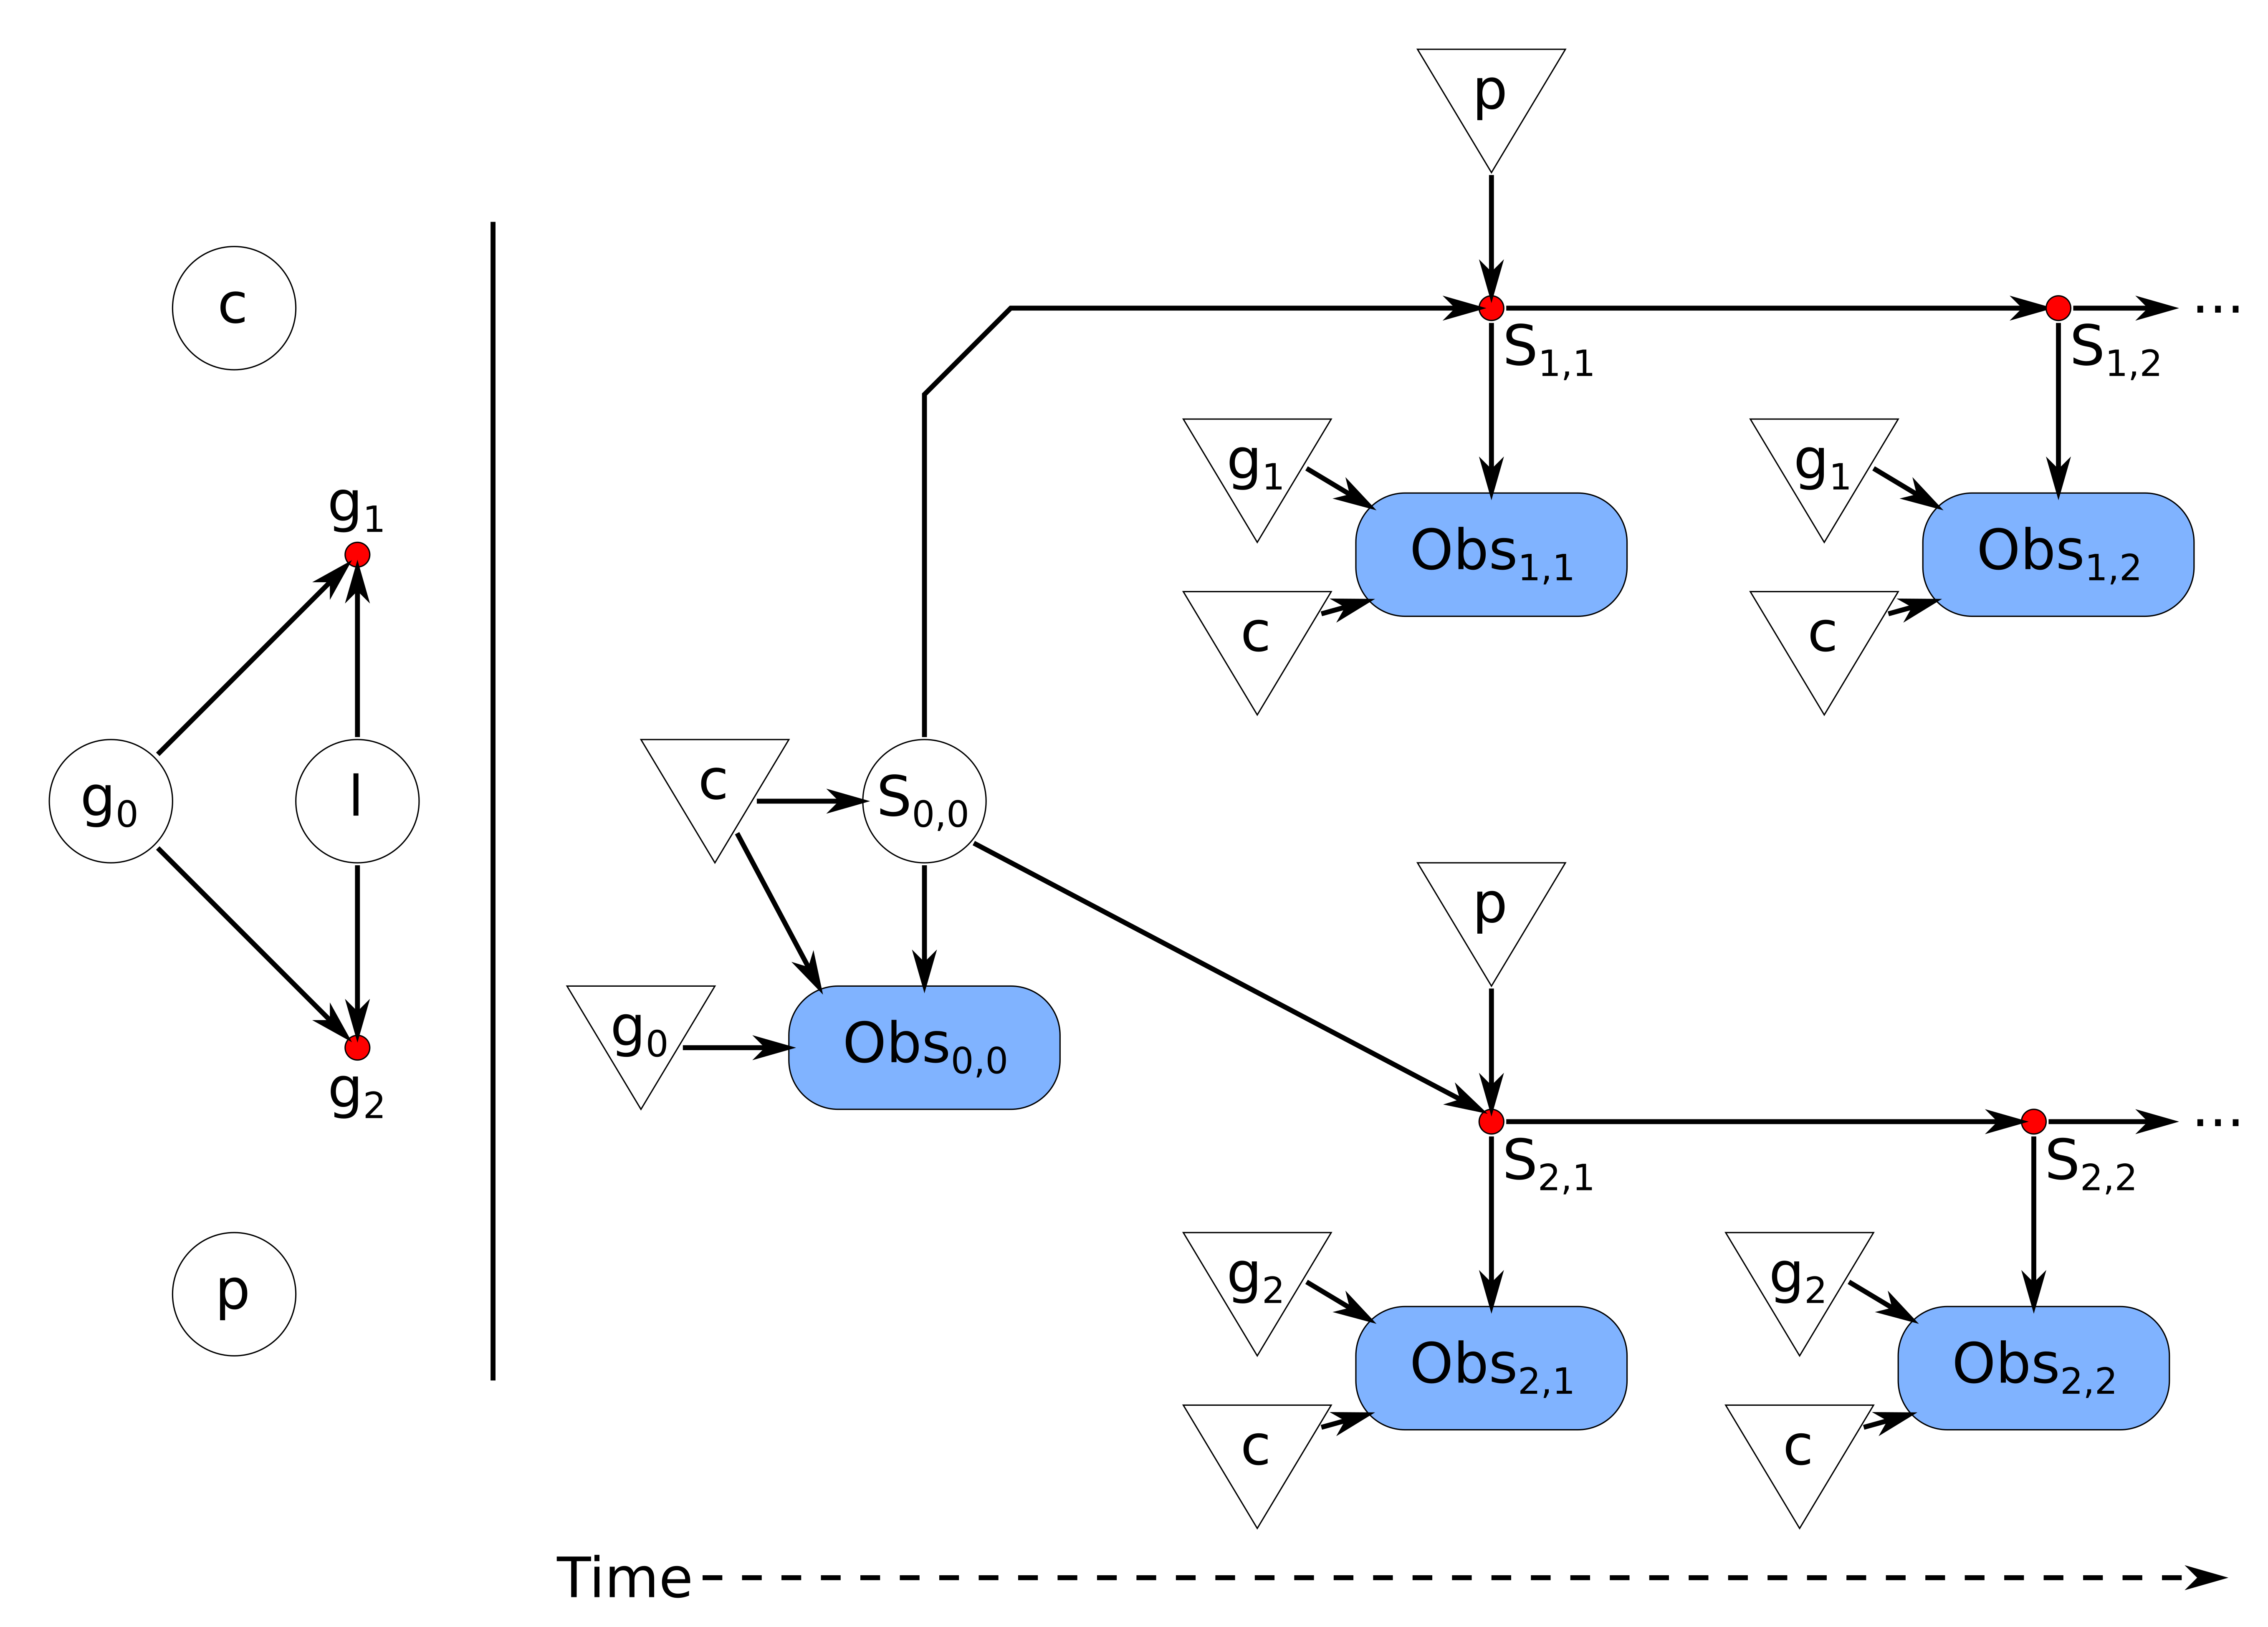
\includegraphics[width=0.8\linewidth]{figs/bayes-net.png}
\end{center}
   \caption{The Bayesian Network for the 2D block model. Hidden random variables 
        are represented as white circles. Deterministic variables are 
        represented as small red dots. Observed variables are represented as 
        light blue ovals. Pointers to other variables in the bayes net are 
        represented as white triangles.}
\label{fig:bayes-net}
\end{figure}

We assume several known constants in the model:

\begin{itemize}
    \item $i_w$: width of the images
    \item $i_h$: height of the images
    \item $M$: number of images
    \item $c_{fps}$: frames per second of the camera
\end{itemize}

We make use of the following hidden random variables:

\begin{itemize}
    \item $c$: the camera
    \item $g_0$: the fracturing object's initial gemoetry
    \item $s_{0,0}$: the fracturing object's initial state
    \item $l$: the fracture partition
    \item $\rho$: the fracture momentum for one of the fragments
\end{itemize}

Which can be represented as a prior in our model as:

$$
p(c, g_0, s_{0,0}, l, \rho) = p(c)p(g_0)p(l)p(\rho)p(s_{0,0}|c)
$$

In a 2D model, the camera, $c$, is greatly simplified. Knowing $i_w, i_h$, it can 
be defined entirely as the boundary of the camera in world space. By assuming 
an aspect ratio that is consistent with the image and keeping two of the 
boundaries (left and bottom) constant, we define the camera in its entirey by 
one boundary. Note that, to ensure the camera does not flip the scene, we 
constrain the top boundary to be greater than 0. In practice, we use a truncated 
normal distribution:

$$
c \sim TruncNormal(\mu_c, \sigma_c, 0, \infty)
$$

$g_0$ can be likewise defined in a simple way. By assuming it is a block that is 
oriented orthogonally to the world basis, we can simply define it in terms of 
its width and height. Again, this creates some constraints. Namely, that both 
width and height must both be greater than 0. Again, we use truncated normal 
distributions for these two quantities, based on priors of the typical size 
of a log used in firewood chopping:

$$
g_0 \sim TruncNormal(\mu_{g_0}, \sigma_{g_0}, 0, \infty)
$$

While we model state in terms of several quantities (position, velocity, angle, 
and angular velocity), our assumptions (1) that the block is oriented 
orthogonally to the world basis and (2) that the block does not move until the 
fracture event happens makes $s_{0,0}$ easy to define. We simply position the 
block based on a distribution centered at the camera's center:

$$
s_{0,0} \sim Normal(\mu_{s_{0,0}}(c), \sigma_{s_{0,0}}(c))
$$

The fracture location, $l$, along the width of the initial block entirely determines 
the fracture partition in this model. Its distribution is conditioned and 
constrained on the block's width:

$$
l \sim TruncNormal(\mu_{l}(g_0), \sigma_{l}(g_0), 0, high_{l}(g_0))
$$

Our last hidden variable, $\rho$ (momentum), is a prior that is roughly based on our 
observations from the firewood chopping videos. It is constrained such that 
the blocks move apart and rotate in directions consistent with an axe chopping 
the block in half from above:

$$
\rho \sim TruncNormal(\mu_{\rho}, \sigma_{\rho}, 0, \infty)
$$

Many of the hidden variables are delta functions, since the physics simulation 
progresses deterministically. Namely, $g_1, g_2$, the geometry of the two blocks 
are deltas based on $g_0, l$. Further, the state of each fragment $n$ at each timestamp $m$, $s_{n,m}$, 
progresses according to Euler's Method after the fracture because we assume no 
collision.

\begin{align*}
g_n \sim& Delta(x_{g_n}(g_0, l)) \\
s_{n,1} \sim& Delta(x_{s_{n,1}}(s_{0,0}, \rho)) \\
s_{n,m} \sim& Delta(x_{s_{n,m}}(s_{n,(m-1)})) \\
\end{align*}

The observations are represented as the coordinates of each vertex of each 
block or fragment in the image space with some additional noise. The 
correspondences are known. Intuitively, this can be though of as 
projecting each block or fragment's geometry to world coordinates using the 
state vector for that block and frame, $s_{n,m}$, then to image 
coordinates using $c$. Finally, a small amount IID noise is added to each endpoint in terms of 
the image plane:


$$
obs_{n,m} \sim Normal(\mu(c, g_n, s_{n,m}), \sigma(c, g_n, s_{n,m}))
$$

The likelhood term is thus:

\begin{align*}
& p(obs_{0,0}|c, g_0, s_{0,0}) p(obs_{1,1}|c, g_1, s_{1,1}) p(obs_{2,1}|c, g_2, s_{2,1}) \\
& \Pi_{n > 0} \Pi_{m > 1} p(obs_{n,m} | c, g_n, s_{n,m})
\end{align*}

And the full posterior distribution is:

\begin{align*}
p(c, g_0, s_{0,0}, l, \rho | obs) \propto& p(c)p(g_0)p(l)p(\rho)p(s_{0,0}|c)  \\
                                         & \qquad p(obs_{0,0}|c, g_0, s_{0,0}) p(obs_{1,1}|c, g_1, s_{1,1}) p(obs_{2,1}|c, g_2, s_{2,1}) \\
                                         & \qquad \Pi_{n > 0} \Pi_{m > 1} p(obs_{n,m} | c, g_n, s_{n,m})
\end{align*}

where $obs$ denotes the set of all observations, indexed over $N, M$.

\subsection{Inference}
\label{inference}

In general, an inference strategy for fracture would require additional model 
selection components. However, we have simplified the model to be a binary 
fracture model where the fracture occurs between the first and second frames of 
the video sequence. This means that the dimensionality of the joint probability 
space is constant, and no model selection is necessary.

Since there is little model noise and thus low uncertainty, given a set of 
observations, we are interested in finding a MAP estimate.

We turn to a straightforward Metropolis-Hastings approach and several variations 
thereof. We begin with a random walk Metropolis algorithm which samples over 
the hidden variables defined in \ref{approach}. The simplicity of Metropolis-
Hastings can result in several problems, however. First of all, over a posterior 
space of so many variabes and such small observation noise, the optima have very 
steep peaks. The vast majority of the posterior space has very low probability 
with several optima with high probability, which, in our model, are very far 
away from each other. 
This makes choosing the standard 
deviations of the proposal distribution a tradeoff between getting caught in local 
optimum (too low) and an extremely high rejection rate (too high). In other 
words, no matter which standard deviation chosen for the random walk Gaussian 
proposals, the algorithm will have some issues in a multi-modal space.

In addition, due to the cyclic 
nature of angular velocity and the fact that the model is defined in terms of 
momentum, not angular velocity, multiple angular velocity values can result 
in the same observations. Intuitively, if a block is rotating at some value, 
$\Delta$, then that same block rotating at $2\pi + \Delta$ would also result in 
the same observations. Though the joint probabilities of these will be different 
due to our model priors, this does create a multi-modality in our posterior 
space.

To attempt to resolve the multi-modality, we turn to several variations of 
Metropolis-Hastings. First of all, we note that, for samples that get caught in 
local optimum, the block's volume variables are tightly coupled to the momentum 
variables. This makes sense, as velocity, which is a function of volume and 
momentum in this model, is much more closely related to the observations. To 
attempt to decouple momentum and volume, we devise a random-walk sampler which 
samples over velocity and angular velocity rather than momentum and angular 
velocity. Intuitively, this can be seen as 

Another technique to deal with the multi-modality is to simply constrain the 
space over which the sampler can walk. In other words, we can reject samples 
which exhibit an angular velocity that is too high. While such samples 
technically have support, their angular momentum is too high given our model 
priors. Since this technique does not allow the chains to explore the full 
posterior space with valid Metropolis-Hastings proposal probabilities, this 
technique is no longer a valid sampling strategy in theory. In practice, we 
would like a MAP estimate, which this strategy may very well achieve. We explore such a 
constrained sampling approach in 
\ref{experiments-eval}, where we constrain angular velocity to be less than $2\pi$.

Lastly, we augment the Metropolis-Hastings random walk with simulated annealing. 
Our hope is that the samples will have time to explore the space more easily 
when the temperature is high and eventually get "locked" into the global 
optimum when the system cools enough.

\section{Experiments and Evaluation}
\label{experiments-eval}

We present the results of several experiments using the random walk 
Metropolis algorithm and the various modifications discussed in \ref{inference}. 
Wompare the results of our approach with a baseline of gradient descent over 
the log posterior space. We evaluate results in terms of log probability in the 
joint probability space.

\subsection{Naive Random Walk Metropolis}
\label{random-walk-metropolis}

Initially, we were interested in trends between various datasets and finding 
the best proposal distributions for the random walk Metropolis algorithm. We 
began by generating 16 synthetic datasets and running 16 MCMC chains for each 
of the datasets. We measured the log probabilities of each chain in the joint 
probability space over the course of 1,000,000 iterations. We discovered that the 
mixing time was very high and the rate at which the samples mixed slowed as the 
chains progressed. This is likely a result of the model's Gaussian distributions. 
As the samples approach the peaks of the posterior distribution, the slopes of 
those peaks become more gradual due to the model's Gaussian distributions. We 
noticed a trend of chains getting 
caught in local optima for each dataset, even with tuned proposal distributions. 
This illustrates the tradeoff of random walk Metropolis proposals between 
getting caught in local optima vs having an extremely high rejection rate. We 
found that the best proposal standard deviations were roughly 0.015 times the 
expected value of the standard deviations of each of the eight hidden random 
variables. the A 
representative dataset can be found in Figure \ref{fig:random-walk-metropolis-dataset-2}.

\begin{figure}[t]
\begin{center}
   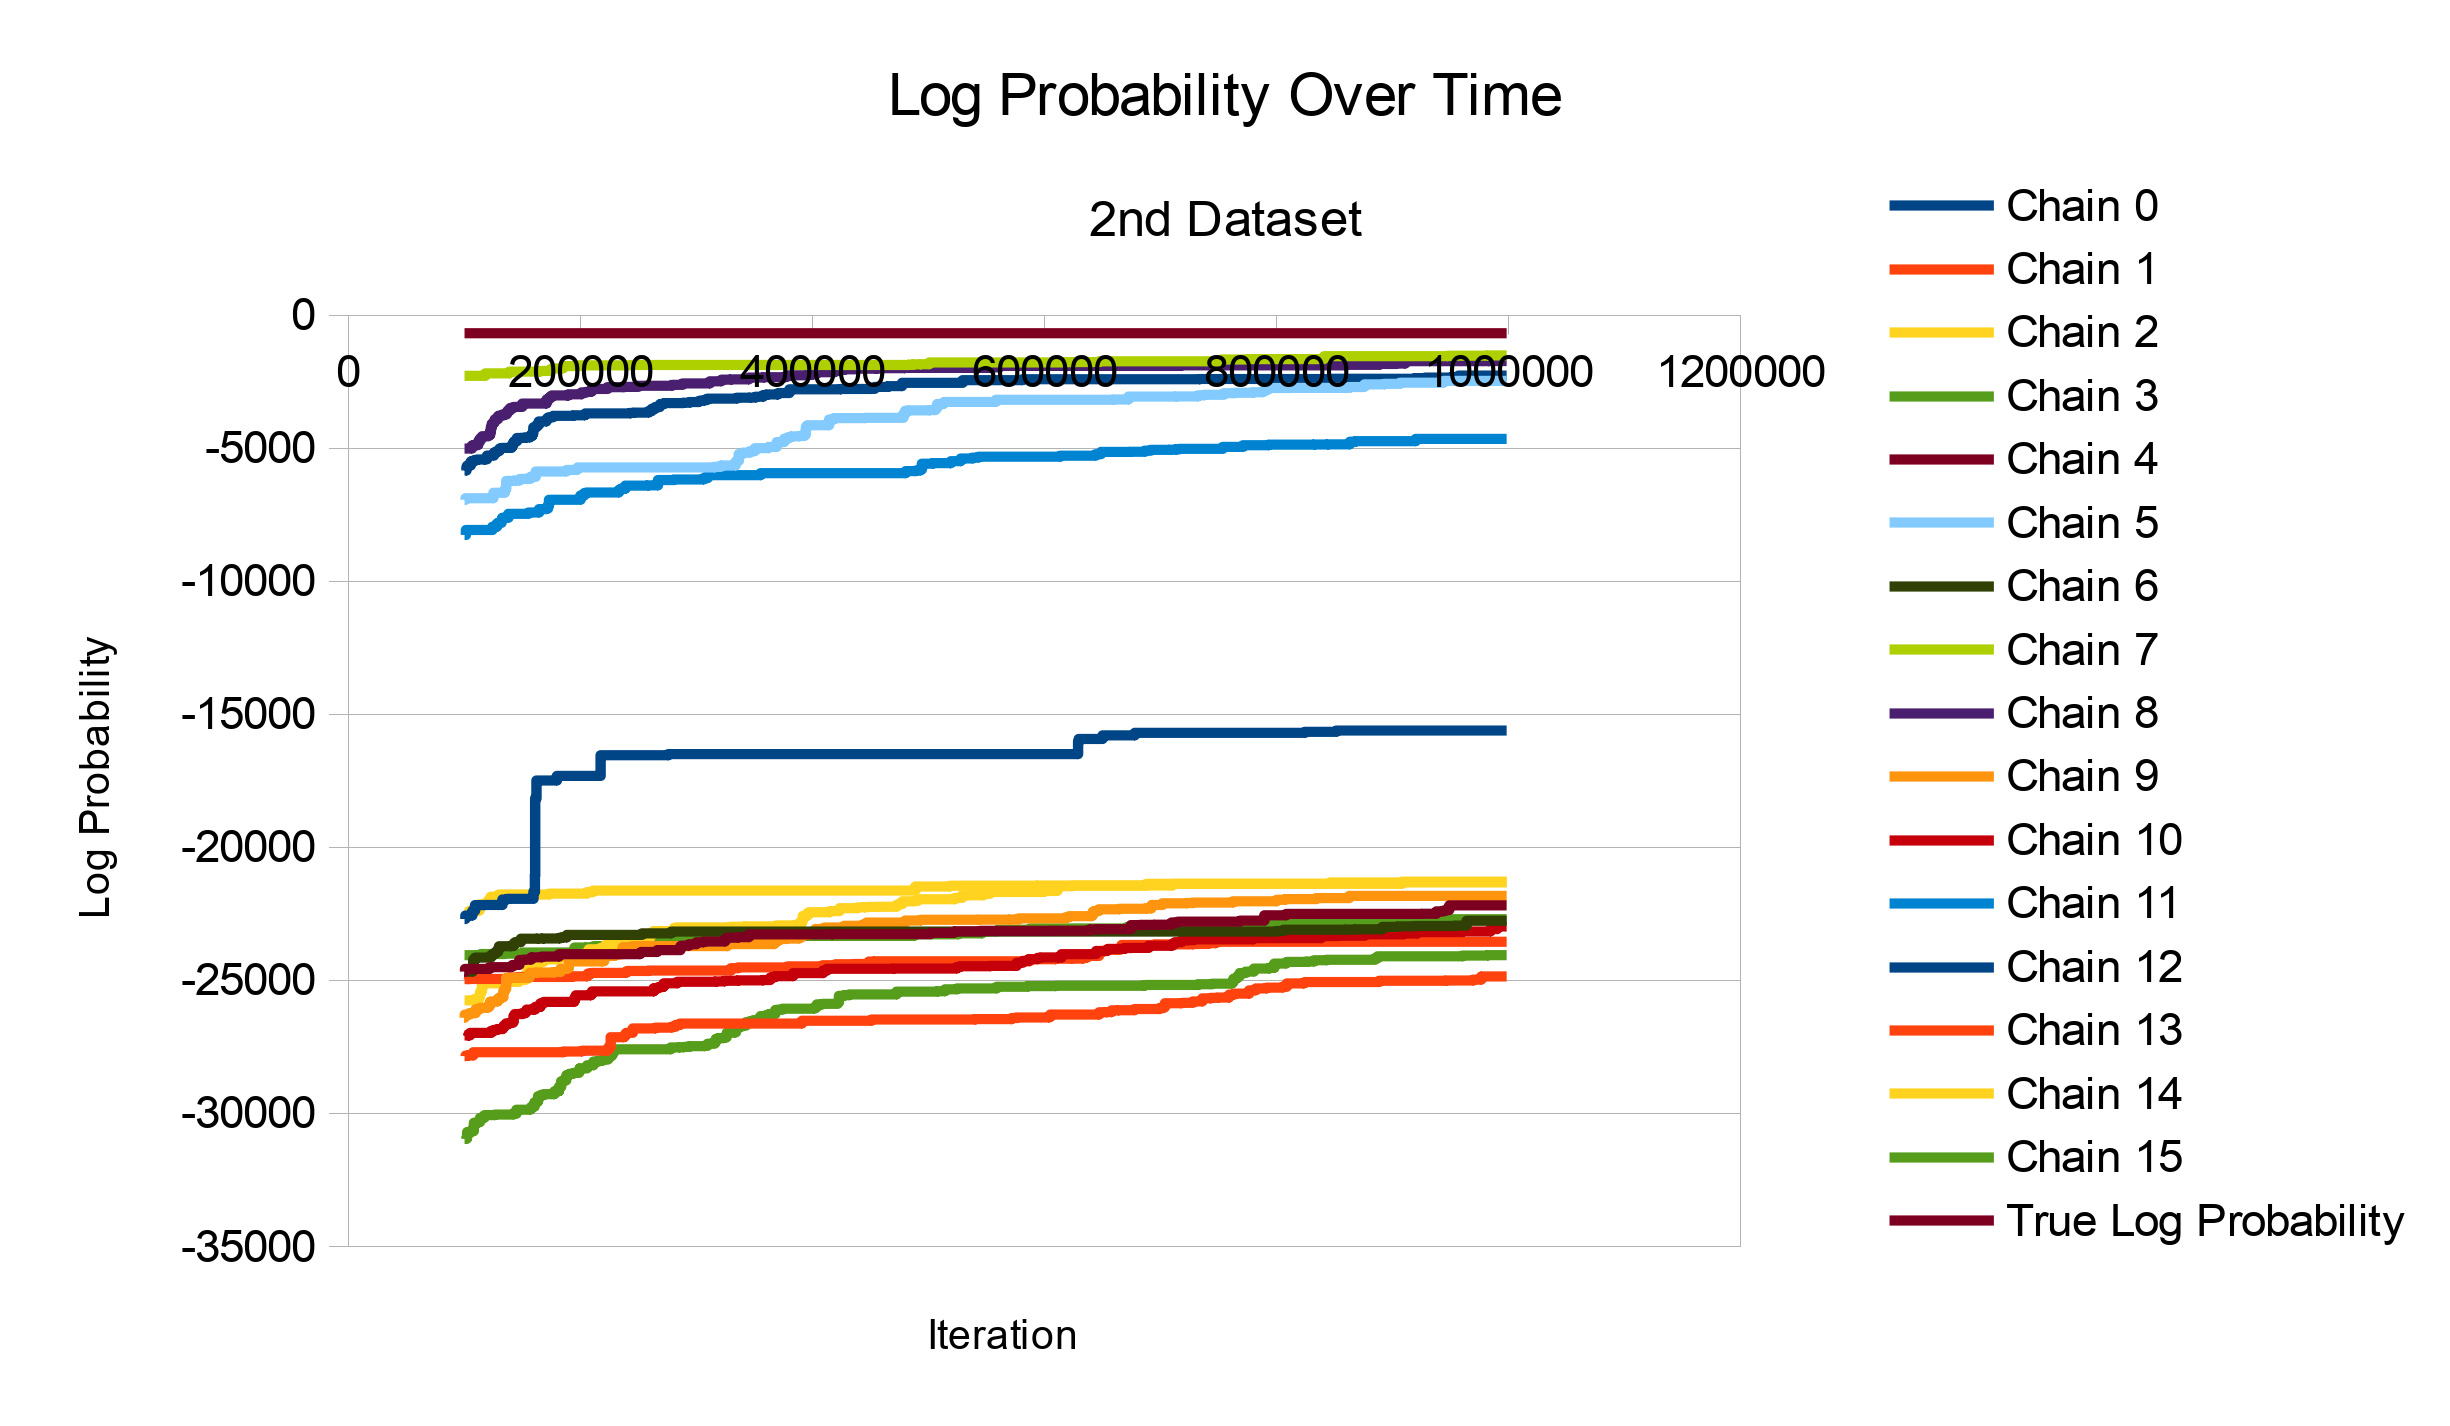
\includegraphics[width=0.8\linewidth]{figs/random-walk-metropolis-dataset-2.png}
\end{center}
   \caption{16 chains of Random walk Metropolis over a dataset. Results are 
        given in terms of log probability over the joint probability space over 
        time (iterations of the chains).}
\label{fig:random-walk-metropolis-dataset-2}
\end{figure}

We noted that, for some datasets, the chains were able to jump to the global 
optimum in a reasonable amount of time, as in figure \ref{fig:random-walk-metropolis-jump-quick}

\begin{figure}[t]
\begin{center}
   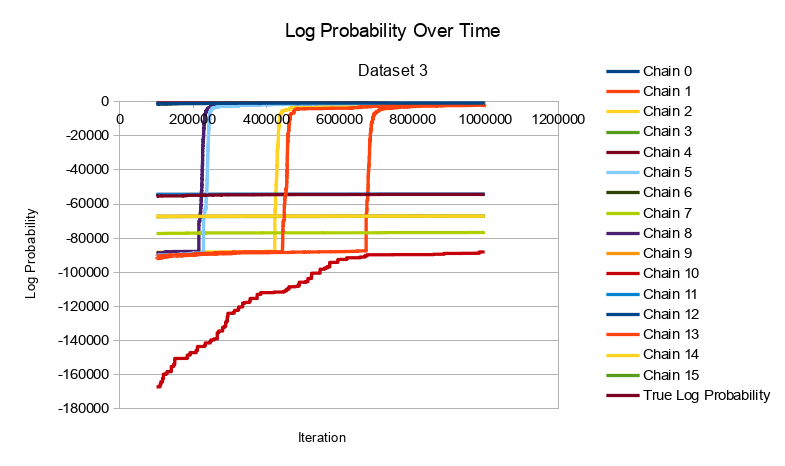
\includegraphics[width=0.8\linewidth]{figs/random-walk-metropolis-jump-quick.png}
\end{center}
   \caption{For some datasets, some chains are able to jump out of the local optima 
        in a reasonable amount of time.}
\label{fig:random-walk-metropolis-jump-quick}
\end{figure}

We examined a specific dataset and its random walk Metropolis chains to see what 
was causing the local optima. For this dataset, we found that the chains were 
not able to jump to the global optimum until much later iterations (1,500,000 - 4,000,000). 
These results can be found in Figure \ref{fig:random-walk-metropolis-jump-slow}.

\begin{figure}[t]
\begin{center}
   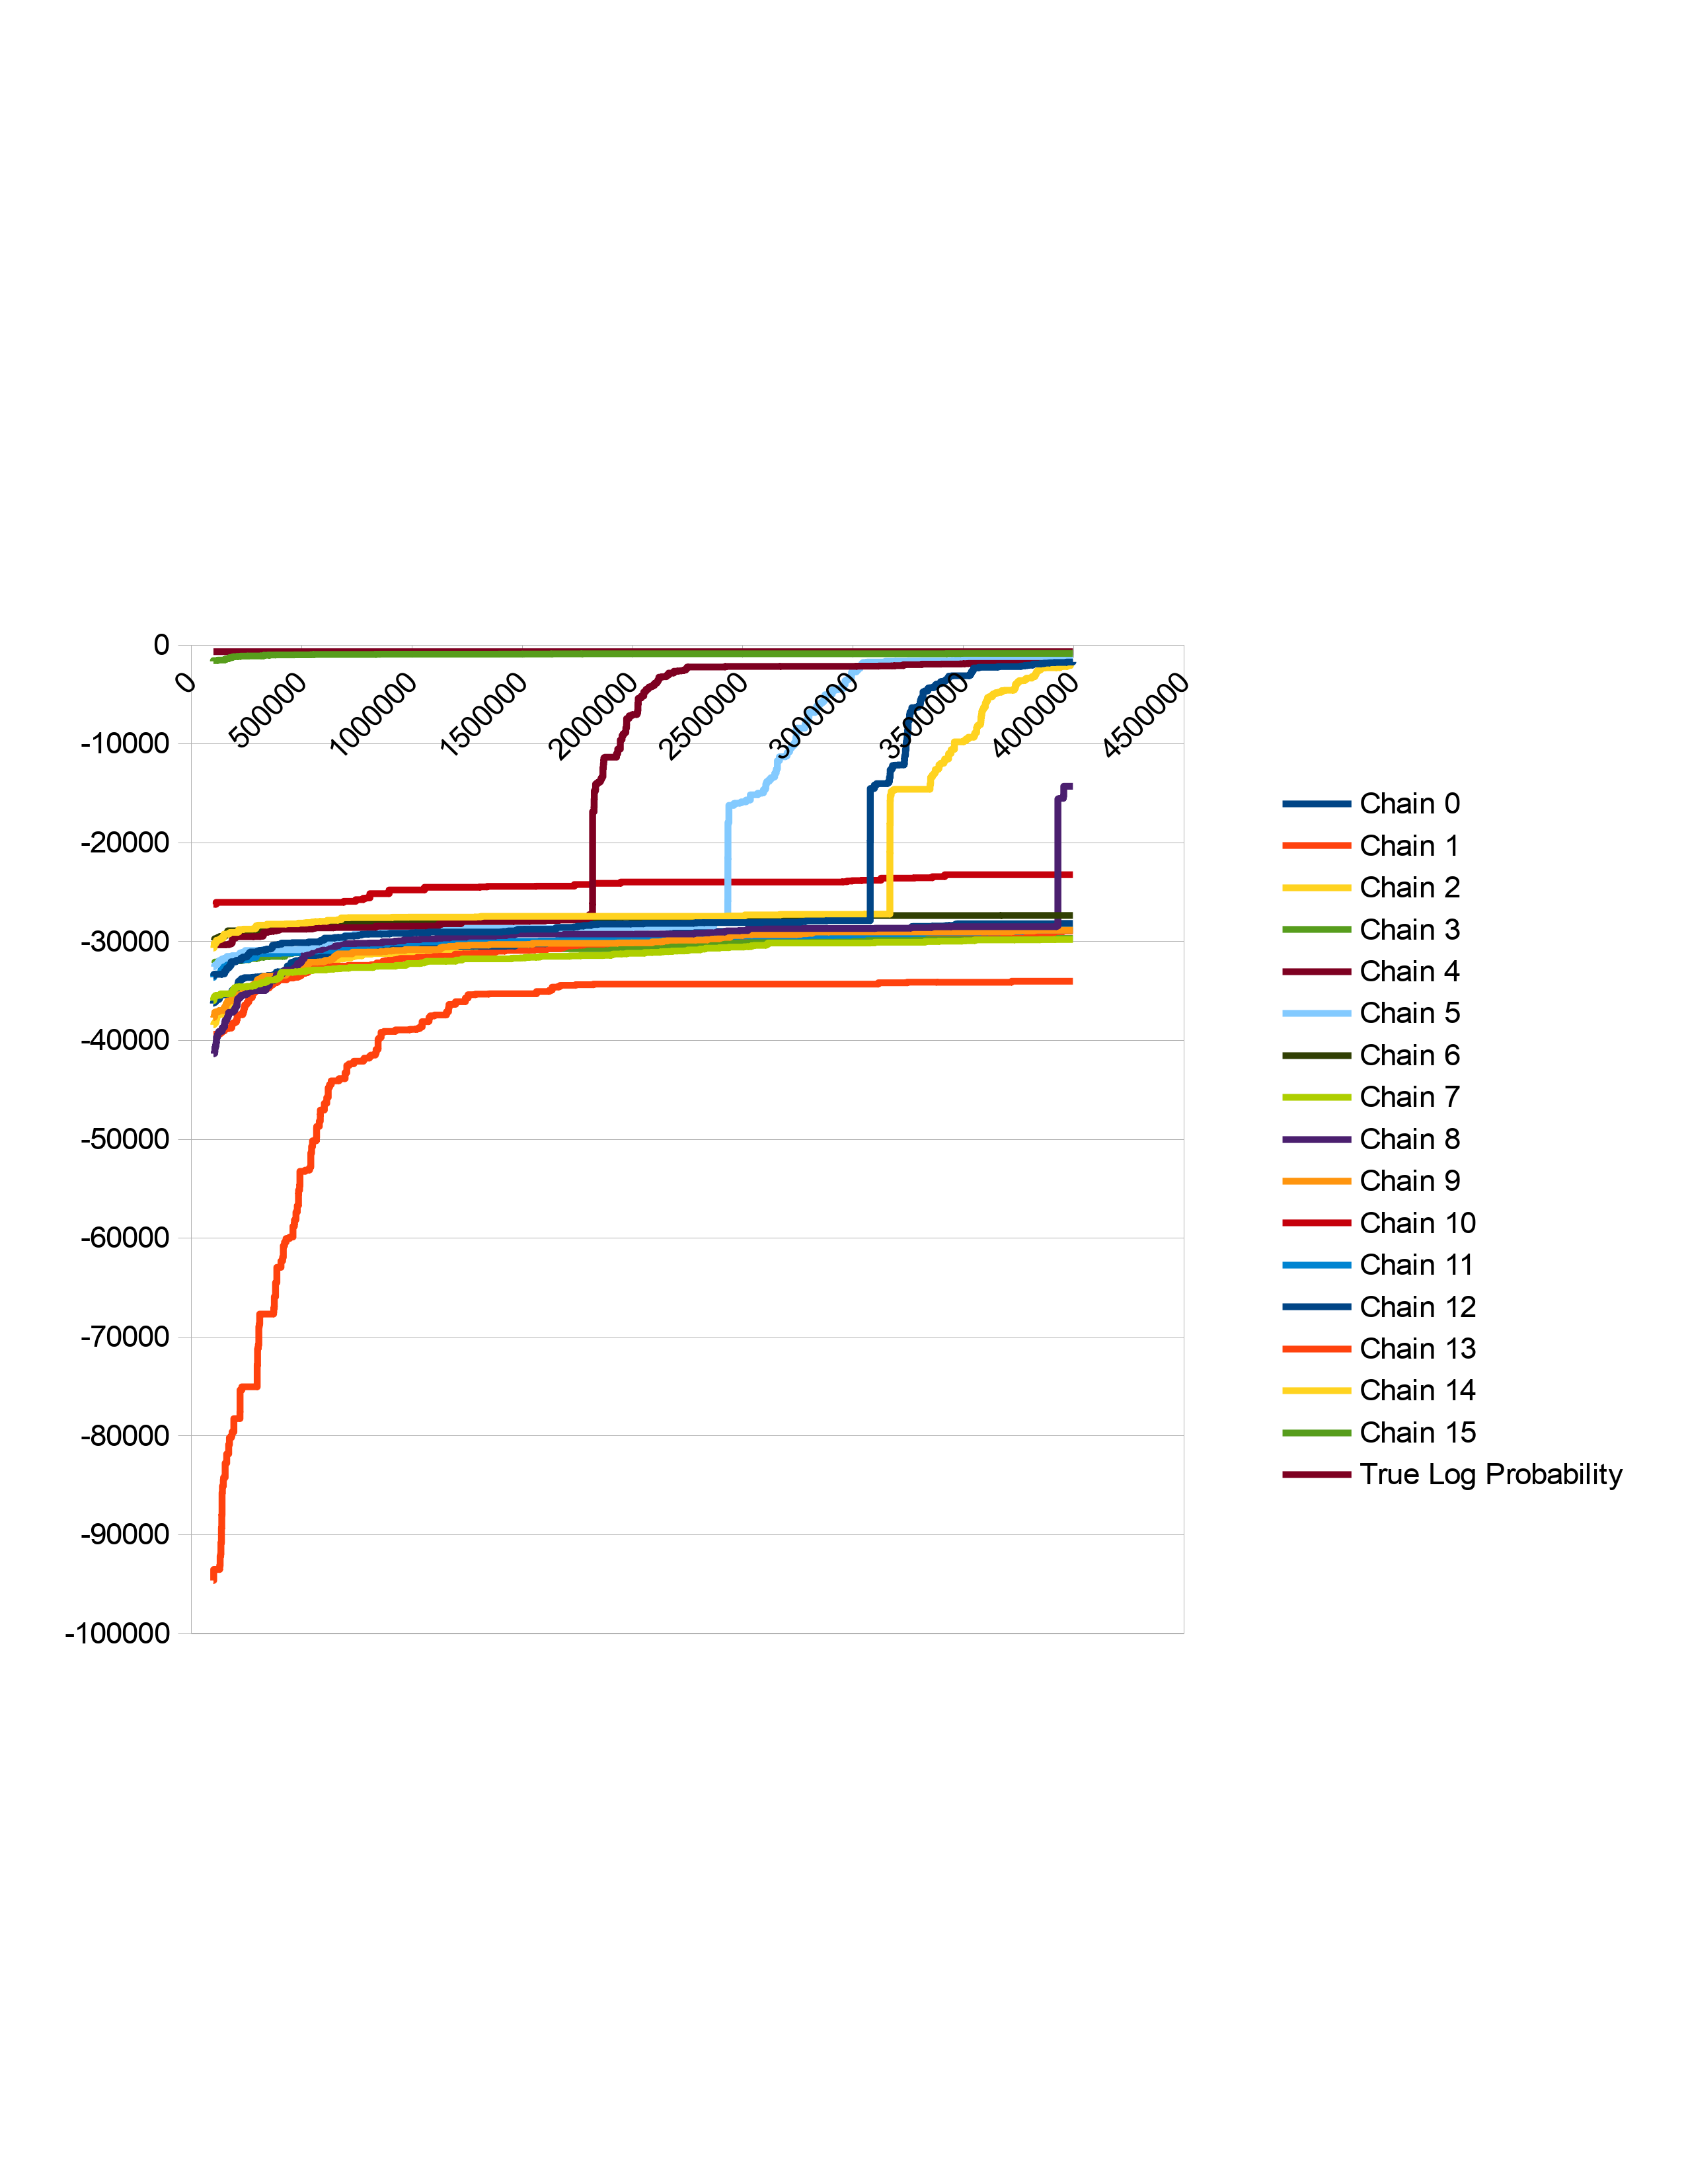
\includegraphics[width=0.8\linewidth]{figs/random-walk-metropolis-jump-slow.png}
\end{center}
   \caption{For other datasets, chains are not able to jump out of the local 
        optima until much later. This will be the dataset used in future 
        experiments.}
\label{fig:random-walk-metropolis-jump-slow}
\end{figure}

We looked into the hidden random variable assignments of a specific chain that exhibited the "jumping" behavior to 
determine the cause of the local optimum that that chain was caught in. We found 
that the block's volume was tightly coupled with the momentum in this optimum. 
In addition, the angular momentum, in particular, was much higher than the 
ground truth's angular momentum. This lead us to believe that the fragments 
might be rotating at a rate of $2\pi + \Delta$ whereas the ground truth was 
rotating at $\Delta$. The results can be found in Figure \ref{fig:hidden_rvs_over_time}.

\begin{figure}[t]
\begin{center}
   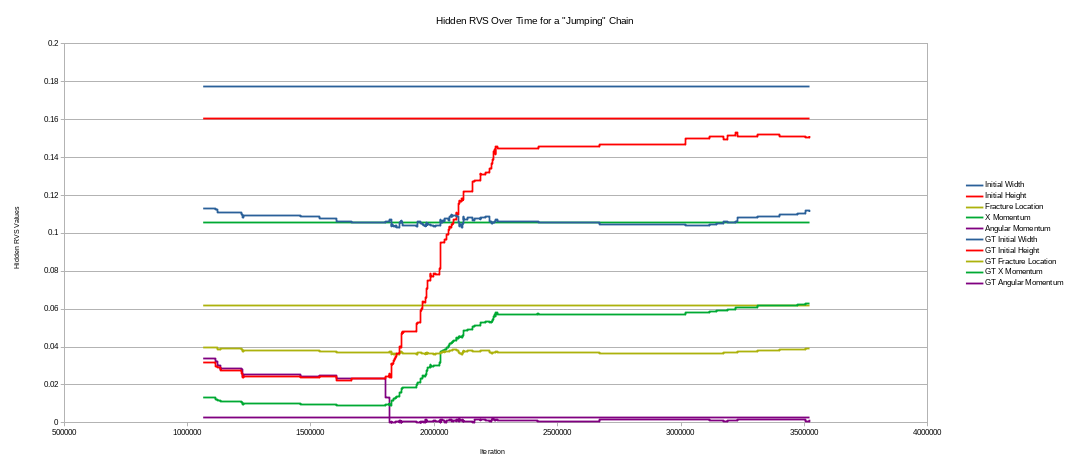
\includegraphics[width=0.8\linewidth]{figs/hidden_rvs_over_time.png}
\end{center}
   \caption{The hidden random variable assignments over time for a chain that 
        jumps out a local optimum. It is clear that the momentum and volume 
        variables (width, height, momentum, angular momentum) are tightly 
        coupled. The chain is finally able to approach the global optimum after 
        the random walk happens to propose a state that is close enough to the 
        global optimum. Note specifically how the angular momentum 
        changes rapidly over the course of several accepted samples.}
\label{fig:hidden_rvs_over_time}
\end{figure}

This led us to make changes in the inference algorithm to attempt to address 
the problems observed here. These are explored in the following sections.

\subsection{Random Walk Metropolis with Velocity Resampling}

Our first modification to random walk Metropolis was to use a proposal 
distribution based not on momentum and angular momentum, but on velocity and 
angular velocity. Our hope was that this would help to decouple the tightly 
coupled volume and momentum in the sampling strategy. Proposal standard 
deviations for these new velocity terms were likewise chosen to be 0.015 times a 
deterministic function in terms of the expected value of momentum and volume. 
With the same 16 initial conditions of the chains, these changes actually 
reduced the ability of the chains to jump out of the local optima. The 
results can be found in Figure \ref{fig:velocity-resampling}.

\begin{figure}[t]
\begin{center}
   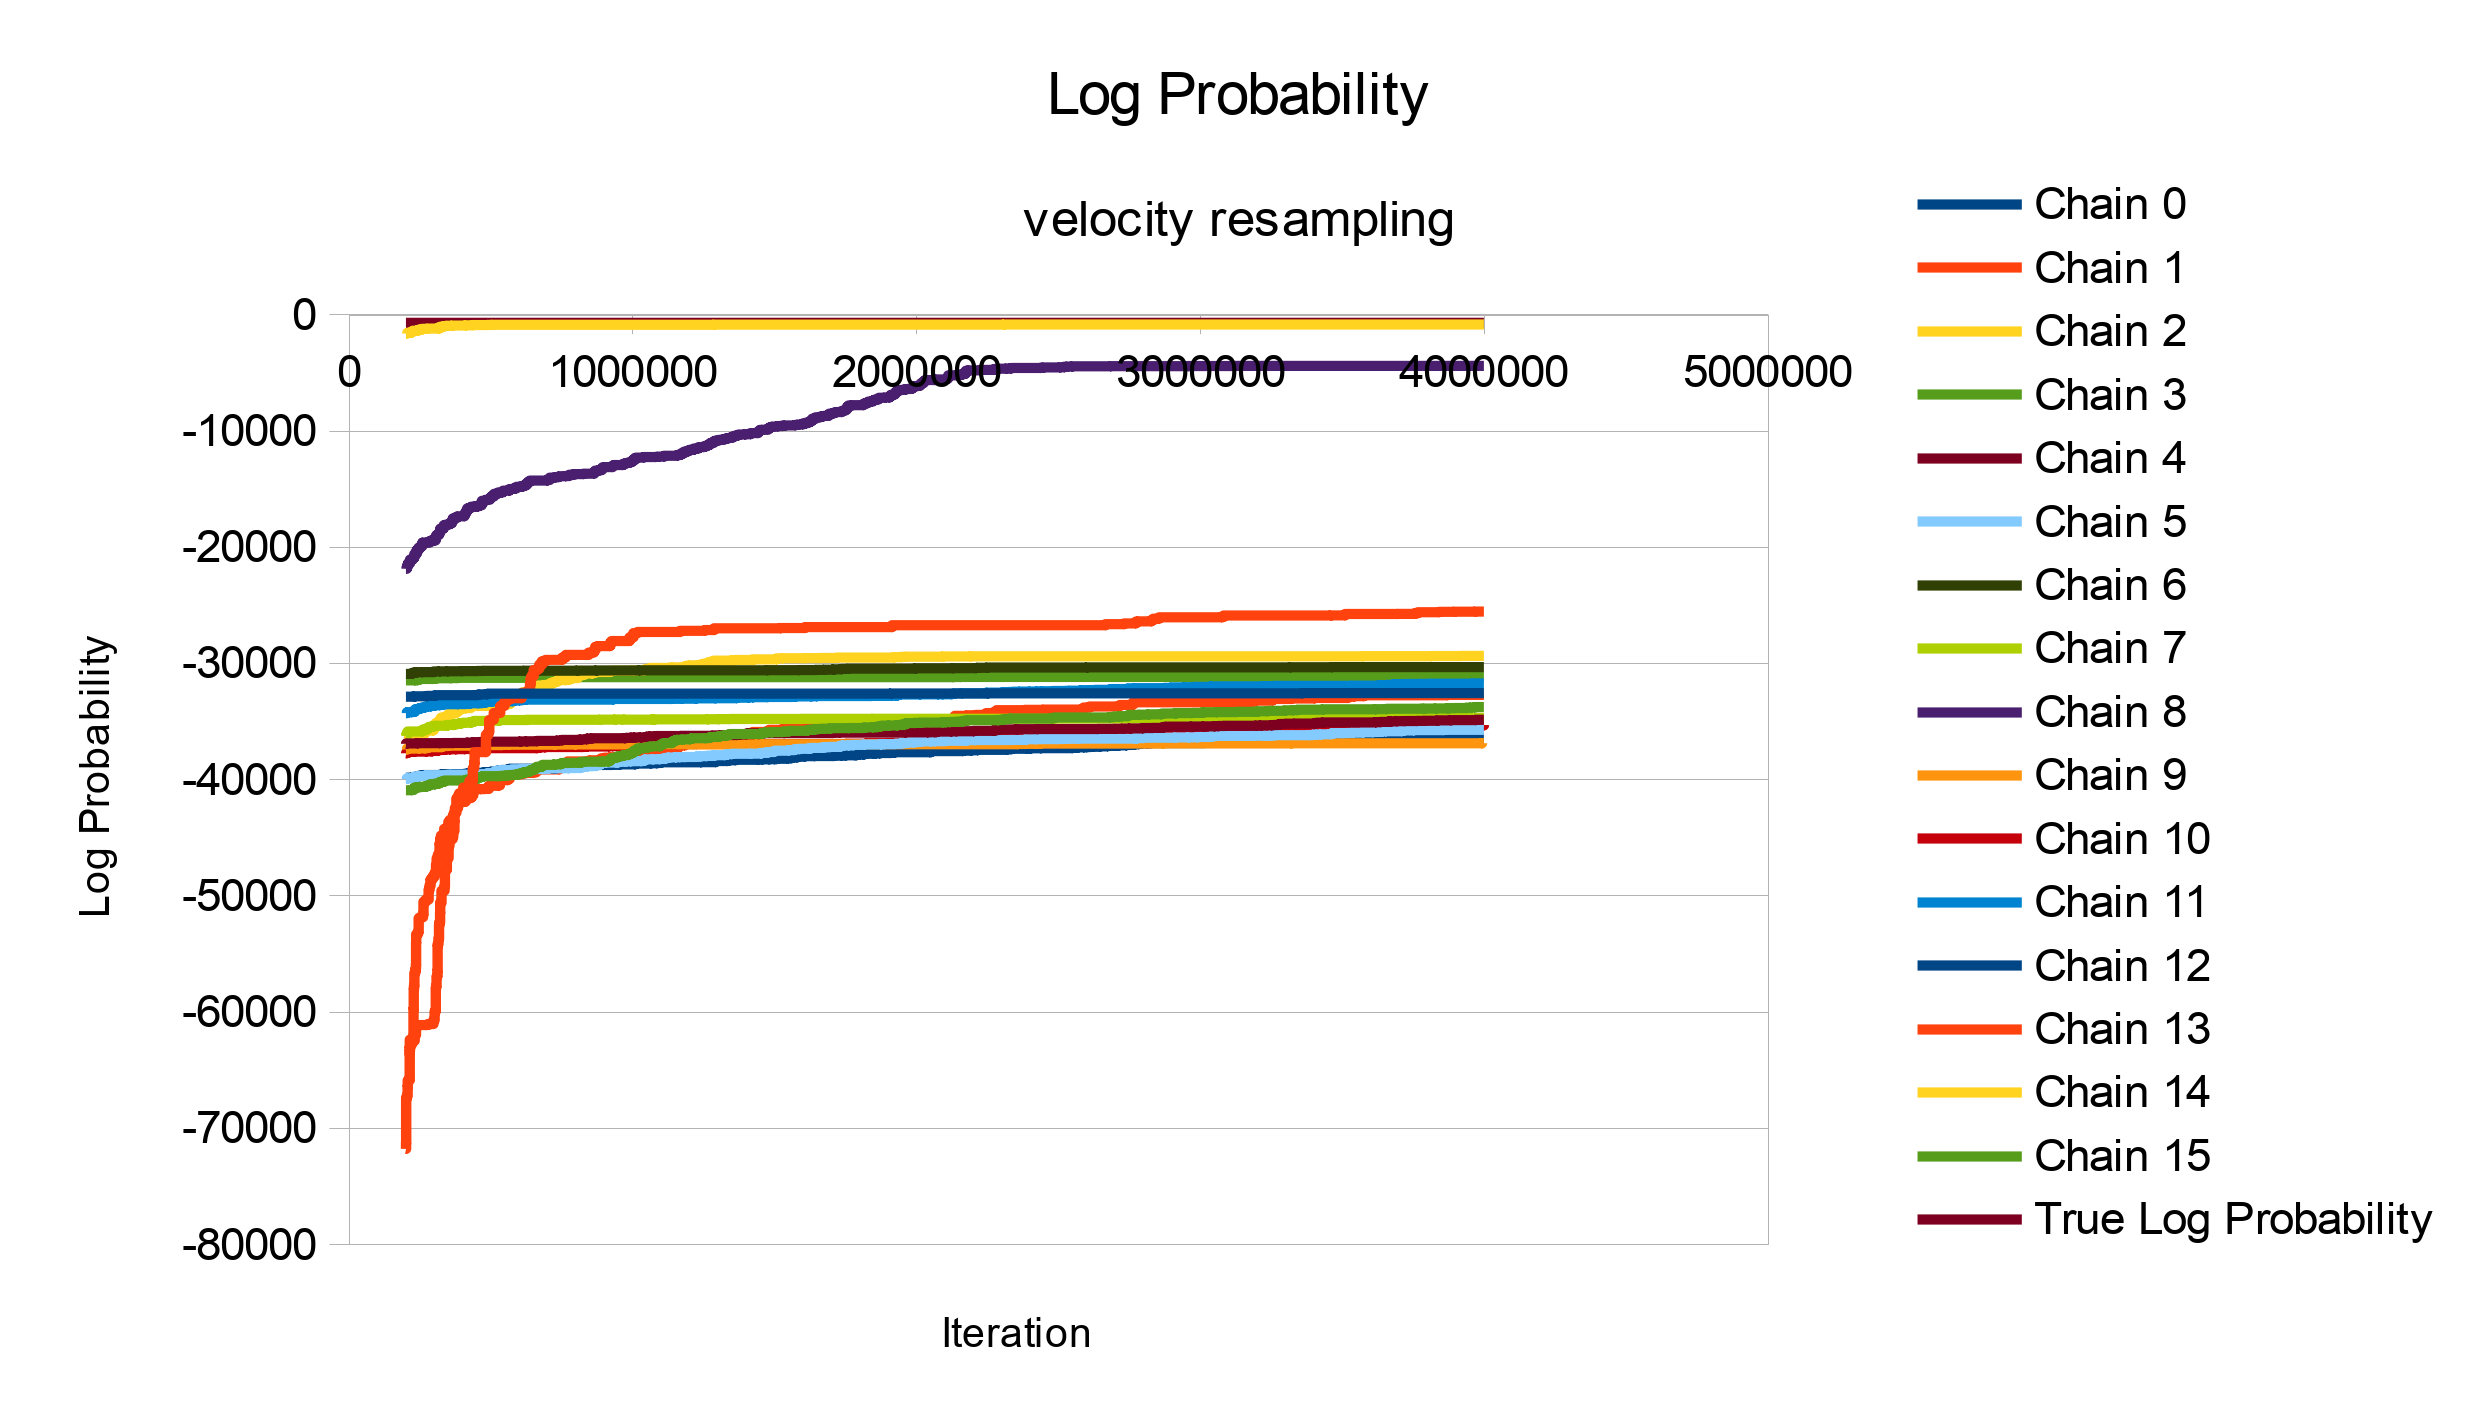
\includegraphics[width=0.8\linewidth]{figs/velocity-resampling.png}
\end{center}
   \caption{16 chains with the same initial conditions as 
        \ref{fig:random-walk-metropolis-jump-slow}. Changing to a velocity 
        sampling scheme reduced the ability of the chains to jump to the global 
        optimum.}
\label{fig:velocity-resampling}
\end{figure}

Our hypothesis of these findings is that the extremely small block sizes present 
in the local optima (see Figure \ref{fig:hidden_rvs_over_time}) were not 
representative of the expected value of volume. This meant that the proposal 
distribution over velocity had a much smaller standard deviation than would be 
needed for the chains to jump to the global optimum. Further experimentation is 
necessary to see if larger standard deviations for the velocity proposals would 
improve the chains' chances of jumping out of local optima.

\subsection{Random Walk Metropolis with Constrained Angular Velocity}

Our hypothesis that the local optima were rotating at roughly $2\pi + \Delta$ 
rather than the ground truth's $\Delta$ rotation rate led us to explore 
constraining the angular velocity to be less than $2\pi$. Note that we resampled 
in terms of momentum (rather than the velocity resampling variation above) to 
test the efficacy of this approach in isolation. This approach did 
not lead to a large change in the 16 initial conditions above. Results can be 
found in Figure \ref{fig:ang-vel-constraint}

\begin{figure}[t]
\begin{center}
   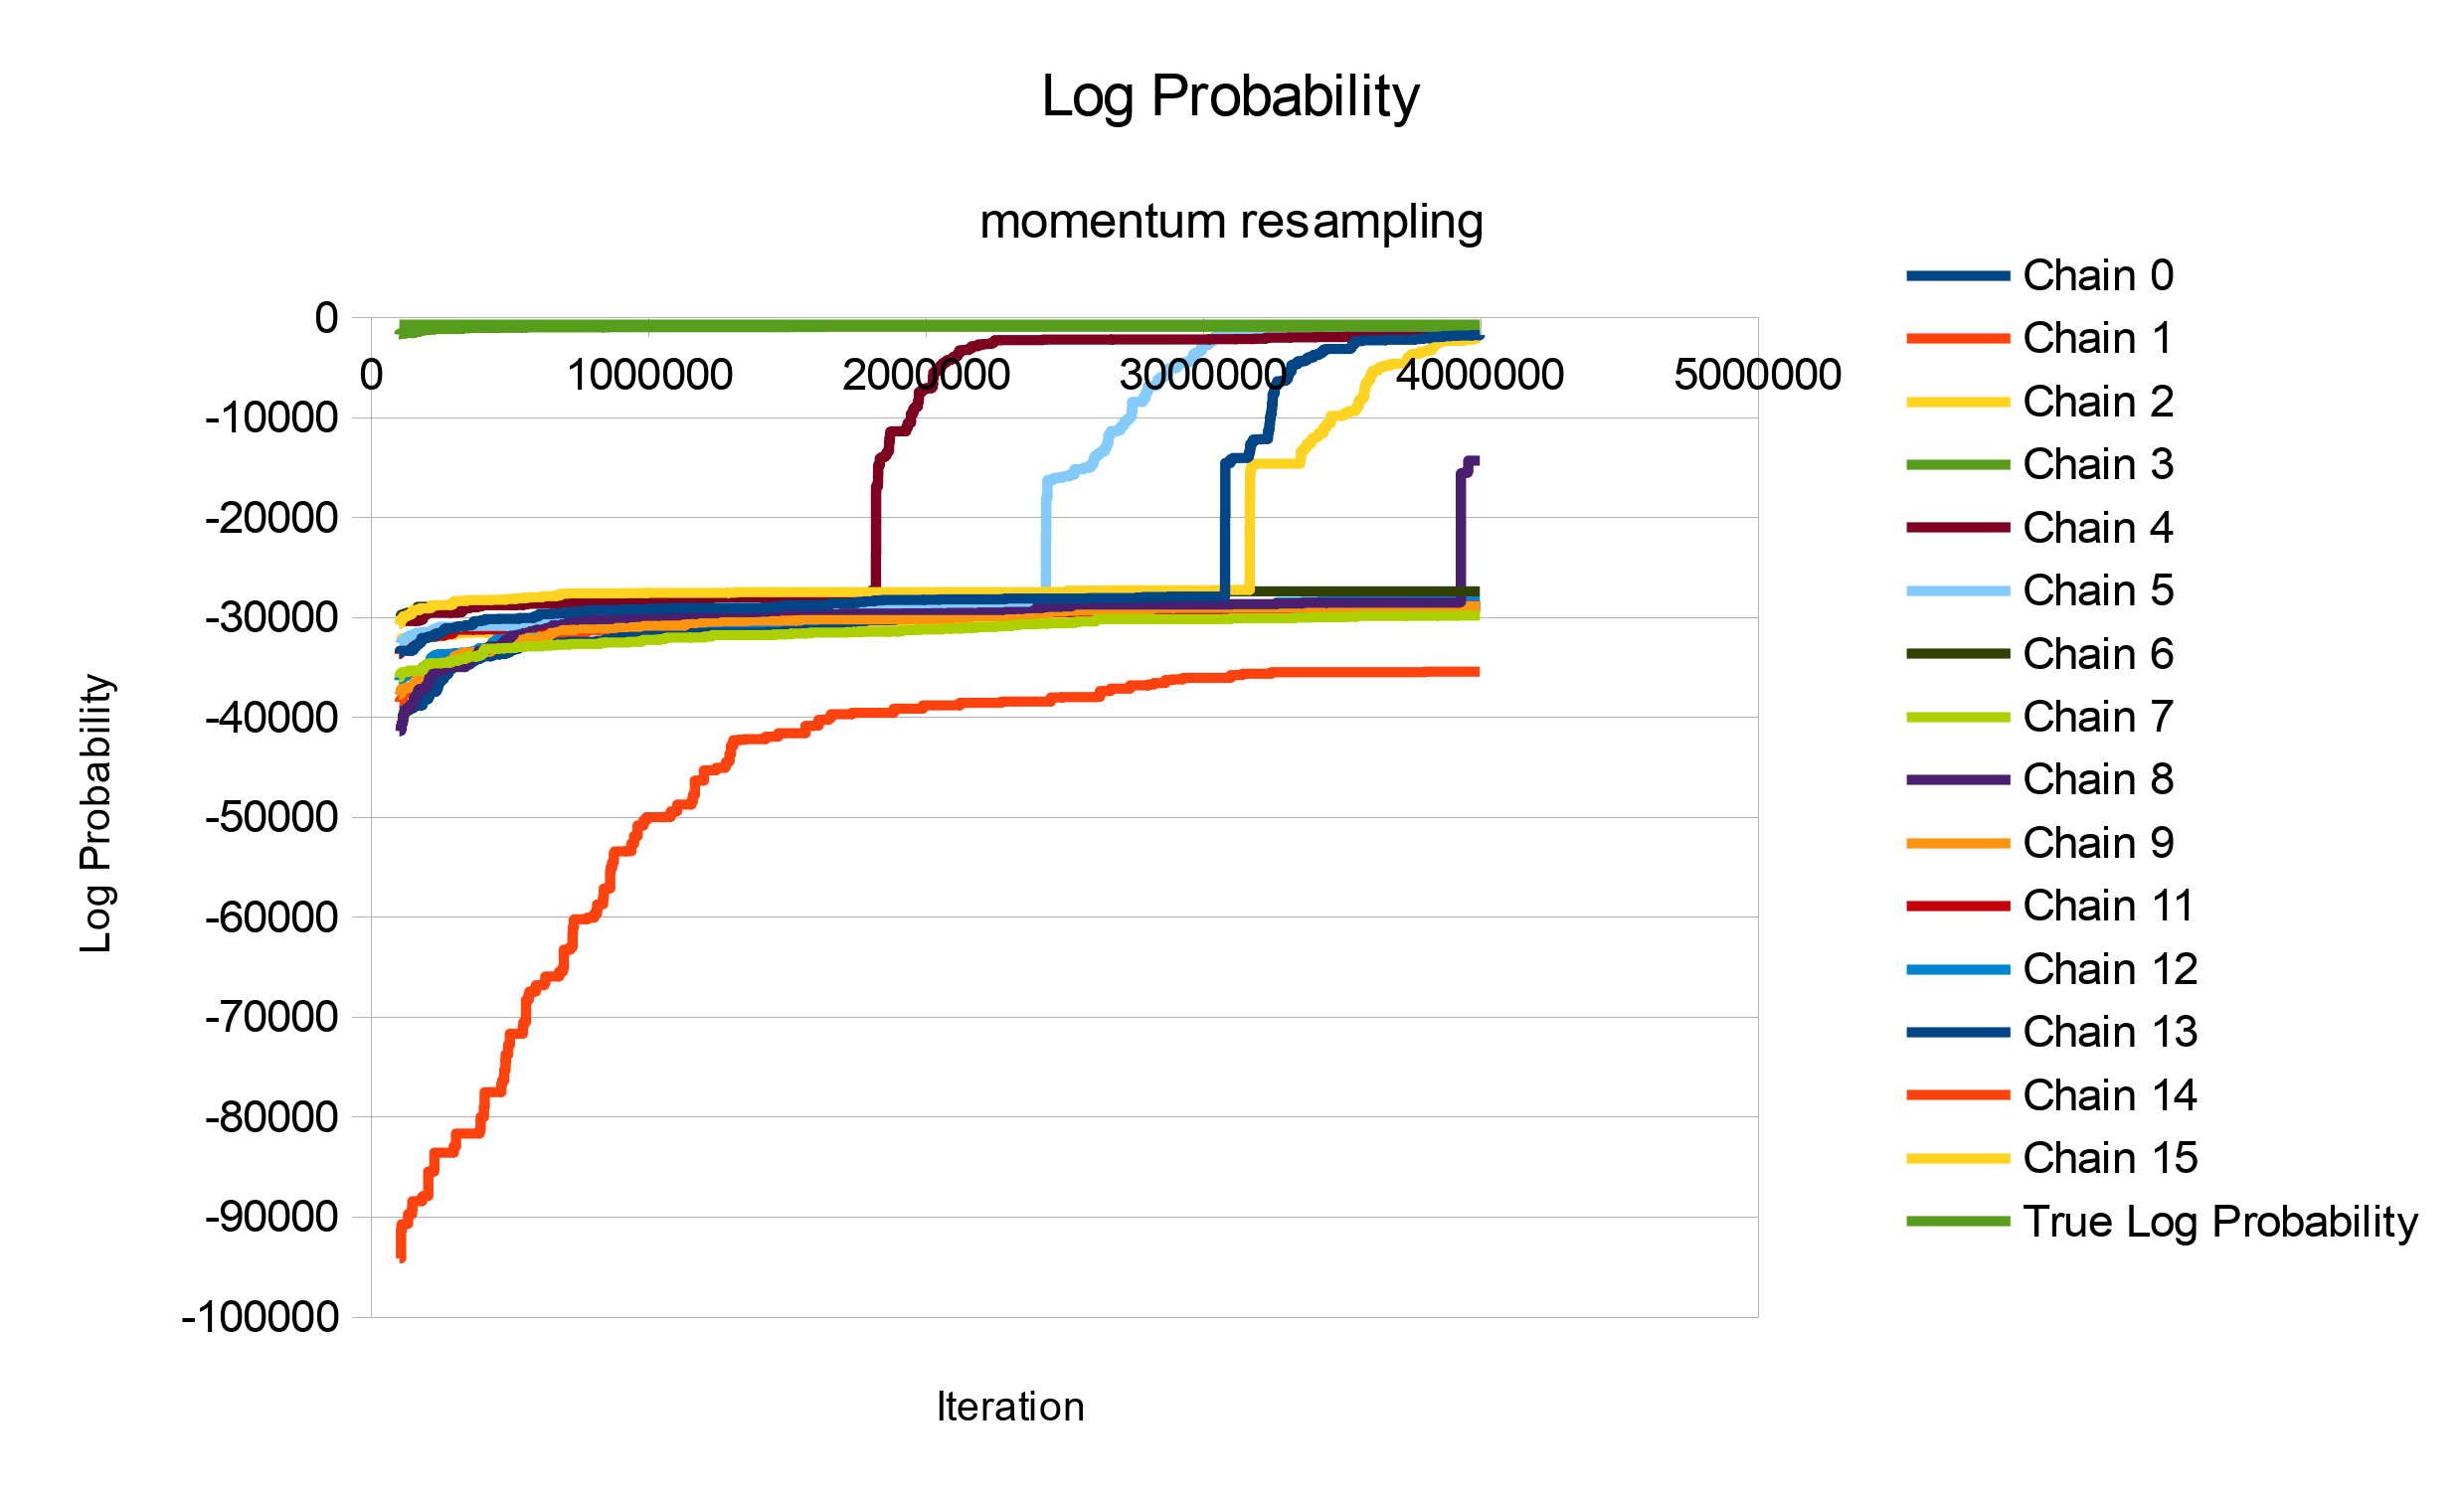
\includegraphics[width=0.8\linewidth]{figs/ang-vel-constraint.png}
\end{center}
   \caption{16 chains with the same initial conditions as 
        \ref{fig:random-walk-metropolis-jump-slow}. Constraining angular 
            velocity to be less than $2\pi$ did not effect much change.}
\label{fig:ang-vel-constraint}
\end{figure}

These results are illuminated after looking into the corresponding angular 
velocity and image sequence produced at the local optimum. In reality, at this 
point, the block 
was rotating a bit faster than $\pi$. While our original hypothesis turned out 
to be incorrect, our revised hypothesis is that, while the 
likelihood term is attempting to pull the chain toward $2\pi + \Delta$, the 
priors on block volume and angular momentum are fighting the likelihood term, 
causing the local optimum to appear at this spot rather than the originally 
hypothesized $2\pi + \Delta$. Further experimentation is needed on selecting 
a good value for the constraint on angular velocity.

\subsection{Random Walk Metropolis with Simulated Annealing}

As simulated annealing has been used many times successfully in the past, we 
turned to augmenting naive random walk Metropolis 
with simulated annealing. Because the posterior space has such steep peaks, we chose 
a starting temperature of 1,000,000 to allow the chains to walk the space more 
effectively at the start. We chose a coefficient, $\alpha$ such that the system 
would be cooled to its original distribution at roughly 1,000,000 iterations. 
($\alpha=0.999986$). This number was chosen heuristically based on the mixing 
rate observed naive random walk Metropolis, which was roughly 500,000 Again, we ran the chains for 4,000,000 iterations. The log  
probability of the chains' final states can be found in Figure \ref{fig:simulated-annealing}.

\begin{figure}[t]
\begin{center}
   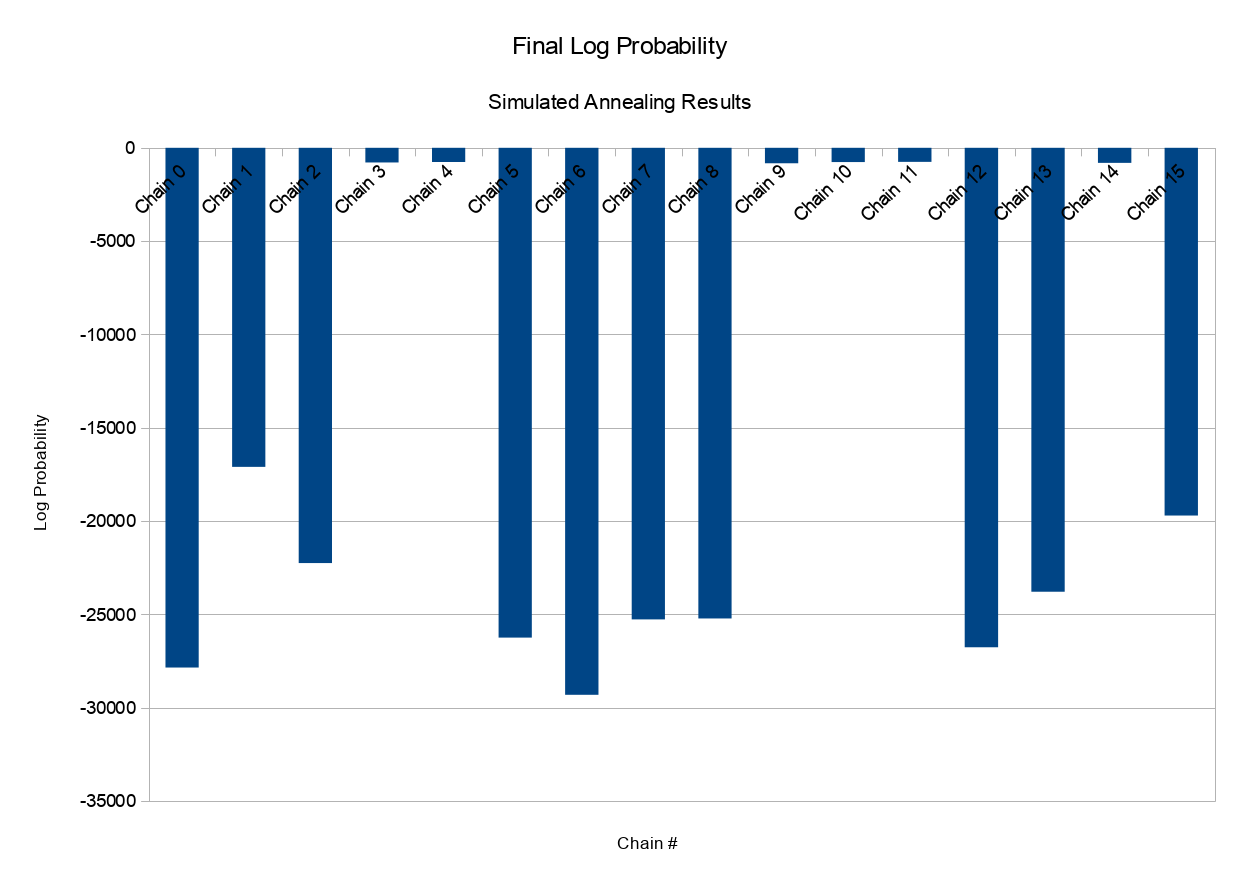
\includegraphics[width=0.8\linewidth]{figs/simulated-annealing.png}
\end{center}
   \caption{16 chains with the same initial conditions as 
        \ref{fig:random-walk-metropolis-jump-slow}, augmented with simulated 
        annealing. More chains were able to reach the global optimum with the 
        same number of iterations as the naive random walk Metropolis 
        algorithm.}
\label{fig:simulated-annealing}
\end{figure}

With the same initial conditions as the previous random walk Metropolis 
experiments, seven chains were able to reach the global optimum, whereas only 
two were able to immediately reach the global optimum in the naive 
implementation. While, in the naive implementation, four other chains were able 
to jump to the global optimum at later states and a fifth was in the process of 
jumping, these results are encouraging. Ideally, we would examine the simulated 
annealing chains over time, but, due to the initial very high acceptance rate, 
the number of stored samples made this untenable. Some aggregation technique is 
necessary to output manageable data to make such a comparison.

\subsection{Gradient Descent over the Log Posterior Space}

For this experiment, we ran a simple gradient descent 16 algorithm over the 
log posterior space. Again, we used the same dataset as the above experiments. 
However, a difference in test apparatus random number generation caused these 
results to begin at different initial conditions to the experiments above.
Experimental results showed that a learning rate of 0.00001 times the normalized 
gradient was a good balance between numerical precision and speed. We represent 
these results in terms of two metrics: for each initial starting condition, the 
final log probability reached (the local optimum found), and the number of 
iterations. This allows us to compare performance in terms of both final results 
and computational effort. Final log probabilities can be found in Figure \ref{fig:grad-desc-log-prob} 
and number of iterations can be found in Figure \ref{fig:grad-desc-iterations}.

\begin{figure}[t]
\begin{center}
   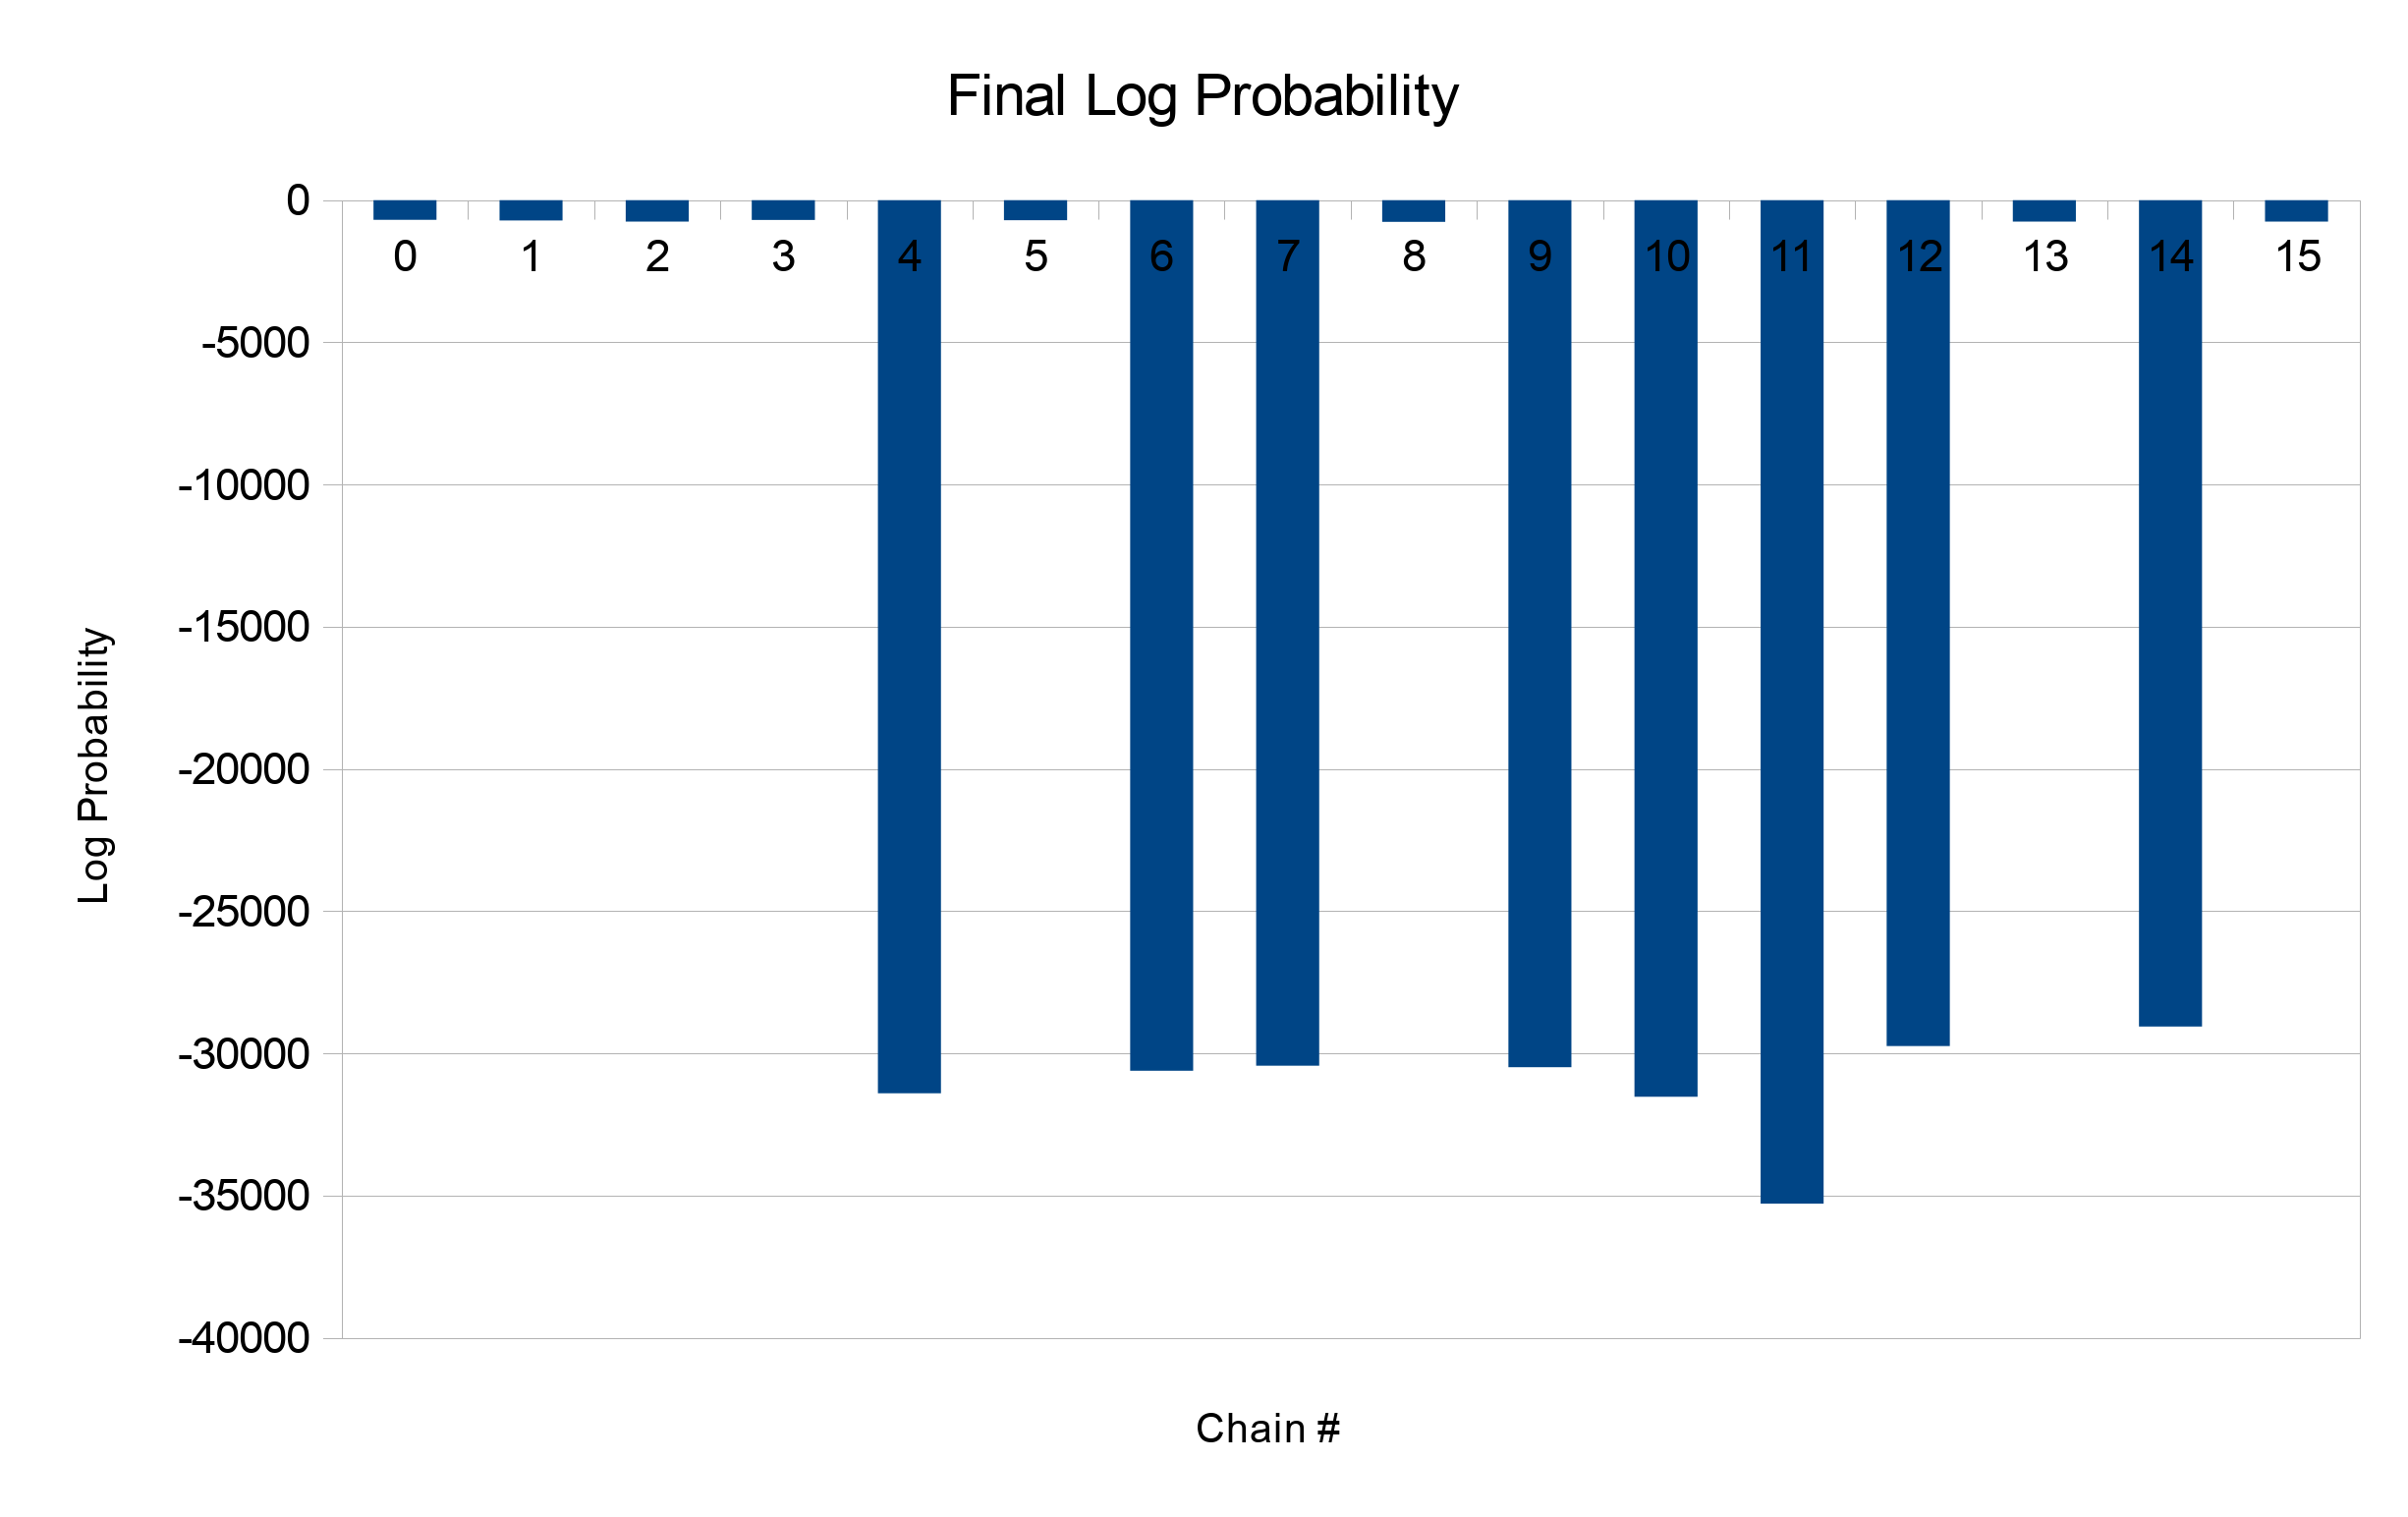
\includegraphics[width=0.8\linewidth]{figs/grad-desc-log-prob.png}
\end{center}
   \caption{The final log probabilities reached from 16 runs of gradient descent, illustrating the multi-modal posterior 
        space. Half of the chains were able to reach the global optimum, while 
        half reached local optima.}
\label{fig:grad-desc-log-prob}
\end{figure}

\begin{figure}[t]
\begin{center}
   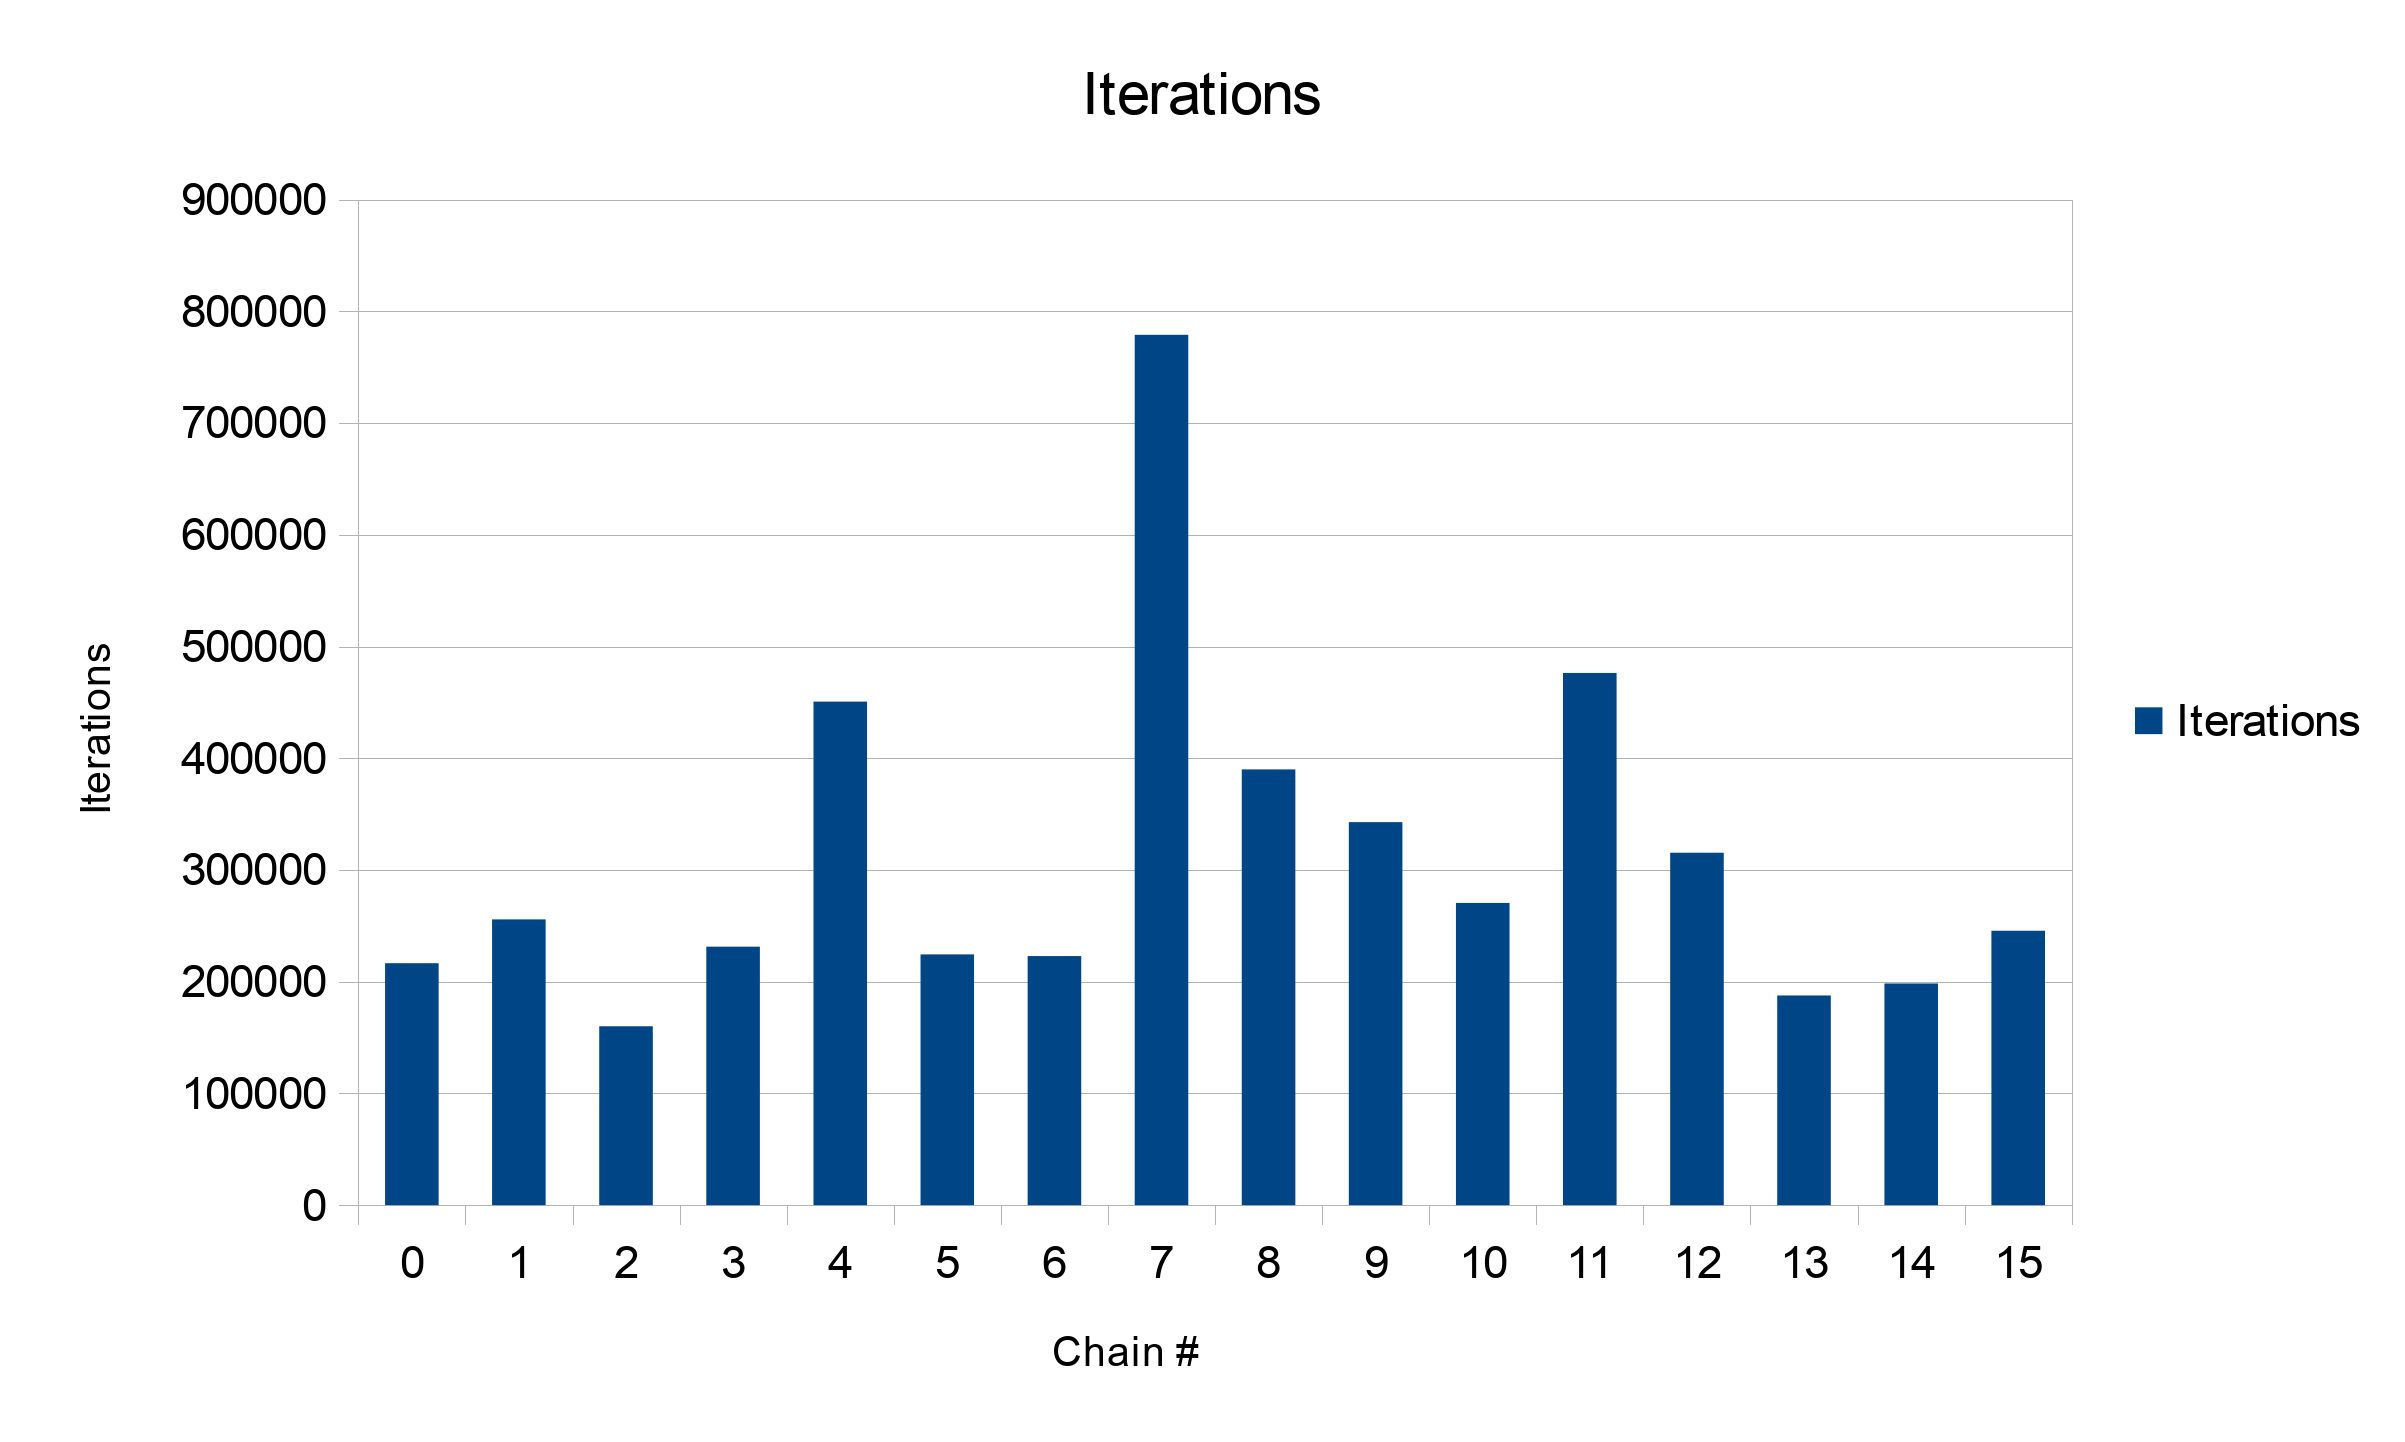
\includegraphics[width=0.8\linewidth]{figs/grad-desc-iterations.png}
\end{center}
   \caption{The number of iterations taken to reach the various optima from 16 
        runs of gradient descent. Compare to the mixing rate of the Metropolis-Hastings chains above.}
\label{fig:grad-desc-iterations}
\end{figure}

The gradient descent results exhibited the same behavior of getting stuck in 
local optima as the random walk Metropolis algorithms. However, gradient descent 
ran in far fewer iterations. While this can be a good indication of 
computational efficiency, it is not entirely a valid metric, as gradient 
descent requires recomputing the gradient at each step, which may be costly, 
whereas Metropolis-Hastings requires sampling from the proposal distributions. 
Further analysis is necessary to obtain a more holistic comparison of 
computational efficiency between 
gradient descent and random walk Metropolis (and variations) above.

\section{Conclusion}

We presented the elements necessary for fracture model and presented some 
simplifying assumptions of our model, based in the real world situation of 
firewood chopping and associated datasets, in 
\ref{req-features-and-simplifying-assumptions}. We presented the state of the 
art (as well as the limitations of these techniques when applied to fracture 
scenarios) of computer vision from the perspectives of tracking and physical 
modeling in \ref{related-work}.
The necessary elements and assumptions allowed us to to define a 
Bayes net with relatively simple geometric priors in \ref{model-definition}. 
Finally, we proposed several inference techniques in \ref{inference} and ran experiments comparing 
those inference techniques to a baseline of gradient descent in \ref{experiments-eval}. 
While this inference task remains difficult, and all 
techniques struggled with the problem of local optima, simulated annealing 
appeared to be the most promising approach, and it approached the performance 
of gradient descent. Further experiments are necessary to explore different 
model definitions and inference strategies to produce the best results for the 
physical modeling of fracture from video evidence.
\par\vfill\par
Now we have reached the maximum size of the ECCV 2018 submission (excluding references).
References should start immediately after the main text, but can continue on p.15 if needed.

\clearpage

\bibliographystyle{splncs}
\bibliography{egbib}
\end{document}
